\chapter{Neural network theory}
\section{Supervised learning}

\begin{definition}[Regression model]
    \label{def:reg_model}
    In machine learning, a regression model $R$ is defined as a mathematical function of the form $R:\mathbb{R}^D\rightarrow \mathbb{R}$ given by
    \begin{equation}
        \label{eq:reg_model}
        R(\vec{x}) = \hat{y} = y + \epsilon
    \end{equation}
    that models the relationship between a $D$-dimensional feature vector $\vec{x} \in \mathbb{R}^D$ of independent (\textit{input}) variables and the dependent (\textit{output}) variable $y \in \mathbb{R}$. 
    Given a particular $\vec{x}$, the model will produce a \textit{prediction} for $y$ which we denote $\hat{y}$.
    Here, the additive error term $\epsilon$ represents the discrepancy between $y$ and $\hat{y}$.
\end{definition}

\begin{definition}[Input space]
    \label{def:input_space}
    The input space $\mathcal{I}_R$ of a regression model $R$ is the set of all possible assignments to the feature vector $\vec{x}$.
    For a feature vector of $D$ dimensions,
    \begin{equation}
        \mathcal{I}_A=\mathbb{R}^D.
    \end{equation}
\end{definition}

\begin{definition}[Labelled dataset]
    \label{def:labelled_dataset}
    A labelled dataset consists of $N$ tuples of the form $\langle \vec{x}_i, y_i\rangle$ for $i=1,\dots,N$.
    For each feature vector $\vec{x}_i$ (a row vector), the corresponding $y_i$ represents the observed output, or \textit{label} \cite{burkov2019}.
    We use the vector
    \begin{equation}
        \label{eq:sup_learn_target}
        \vec{y} = \begin{bmatrix}
            y_1 & y_2 & \cdots & y_N
        \end{bmatrix}\tran
    \end{equation}
    to denote all the labelled outputs in the dataset, and the $N \times D$ matrix
    \begin{equation}
        \label{eq:sup_learn_input_matrix}
        \vec{X} = \begin{bmatrix}
            \vec{x}_1 & \vec{x}_2 & \cdots & \vec{x}_N
        \end{bmatrix}\tran
    \end{equation}
    for representing the corresponding feature vectors.
\end{definition}

\begin{definition}[Supervised learning]
    A supervised learning algorithm for a regression task infers the function $f$ given in (\ref{eq:reg_model}) from a set of \textit{labelled training data} of the form explained previously. 
    We use the vector
    \begin{equation}
        \label{eq:sup_learn_prediction}
        \vec{\hat{y}} = \begin{bmatrix}
            \hat{y}_1 & \hat{y}_2 & \cdots & \hat{y}_N
        \end{bmatrix}\tran
    \end{equation}
    to denote the prediction that $f$ produces for each training sample.
\end{definition}

\section{Artifical neural networks}
\label{sec:ann}
Artifical neural networks (ANNs) take inspiration from the human brain and can be regarded as a set of interconnected neurons. 
More formally, an ANN is a directed graph of $n$ neurons (referred to as \textit{nodes} or \textit{units}) with weighted edges (\textit{links}).
Each link connecting two units $i$ and $j$ is directed and associated with a real-valued weight $w_{i,j}$. 

A particular unit $i$'s \textit{excitation}, denoted $z_i$, is calculated as the weighted sum
\begin{equation}
    z_i = \sum_{j=1}^n{w_{j,i} a_j} + b_i
\end{equation}
where $a_j \in \mathbb{R}$ is another unit $j$'s \textit{activation} and $b_i \in \mathbb{R}$ is the $i$th unit's \textit{bias}.
Notice that in this model, if there exists no link between unit $i$ and a particular $j$ then simply $w_{i,j}=0$ and therefore $j$ will not contribute to $i$'s excitation. 

The unit $i$'s activation is its excitation applied to a non-linear \textit{activation function}, $g: \mathbb{R} \rightarrow \mathbb{R}$. We have
\begin{equation}
    \label{eq:ann_activation}
    a_i = g\left(z_i\right) = g\left(\sum_{j=1}^n{w_{j,i} a_j} + b_i\right).
\end{equation}

\paragraph{Activation functions}
In its original form, \citeauthor{mcculloch1943} defined the neuron as having only binary activation \cite*{mcculloch1943}. 
This means that in our model from (\ref{eq:ann_activation}), we would require $a_i \in \{0, 1\}$ and hence an activation function of the form $g_\text{thres}: \mathbb{R} \rightarrow \{0, 1\}$ which would be defined\footnote{In fact, \citeauthor{mcculloch1943} defined the activation to be zero when $x<\theta$ for a threshold parameter $\theta \in \mathbb{R}$ and one otherwise, but in our model the bias term $b_i$ acts as the threshold.} as
\begin{equation}
    \label{eq:thres_activation}
    g_\text{thres}(x) = \begin{cases} 
        0 & x < 0 \\
        1 & x \geq 0
    \end{cases}.
\end{equation}

Commonly used activation functions in modern neural networks include the sigmoid
\begin{equation}
    g_\text{sig}(x) = \frac{1}{1 + e^{-x}}
\end{equation}
and the rectified linear unit (ReLU)
\begin{equation}
    g_\text{ReLU} = \begin{cases}
        0 & x < 0 \\
        x & x \geq 0
    \end{cases}
\end{equation}
which are depicted in Figure \ref{fig:activation_functions}.
\begin{figure}
    \centering
    \begin{subfigure}{.45\textwidth}
        \begin{tikzpicture}
            \begin{axis}[
                x=0.75cm,
                y=3cm,
                axis lines=center,
                xlabel={$x$}, xlabel style={anchor=west},
                ylabel={$g_\text{sig}(x)$}, ylabel style={anchor=south},
                ymin=0, ymax=1.2,
                xmin=-3.3, xmax=3.3,
                samples=100,
                xtick={-3,...,3},
                ytick={0, 0.5, 1},
                extra x ticks=0
            ]
                \addplot[black] {1 / (1 + exp(-x))};
            \end{axis}
        \end{tikzpicture}
        \caption{Sigmoid}
    \end{subfigure}
    \hspace*{\fill}
    \begin{subfigure}{.45\textwidth}
        \begin{tikzpicture}
            \begin{axis}[
                x=2.25cm,
                y=3cm,
                axis lines=center,
                xlabel={$x$}, xlabel style={anchor=west},
                ylabel={$g_{\text{ReLU}}(x)$}, ylabel style={anchor=south},
                ymin=0, ymax=1.2,
                xmin=-1.1, xmax=1.1,
                samples=100,
                xtick={-1, -0.5, 0, 0.5, 1},
                ytick={0, 0.5, 1},
                extra x ticks=0
            ]
                \addplot[black][domain=0:1] {x};
                \addplot[black][domain=-1:0] {0};
            \end{axis}
        \end{tikzpicture}
        \caption{Rectified linear unit}
    \end{subfigure}
    \caption{Plots of the the two most common activation functions.}
    \label{fig:activation_functions}
\end{figure}
Unlike $g_\text{step}$, these activation functions are differentiable which is an advantage for being able to use gradient descent \cite[p. 729]{russell2010}.

Rectified units do not suffer from the \textit{vanishing gradient effect} \cite{glorot2011}.
This phenomenon occurs with sigmoid activation functions when they reach high saturation, i.e. when the input is significantly far from zero such that the gradient is almost horizontal.
However, the vanishing gradient problem is usually not prevelant in shallow\footnote{Shallow networks refer to ANNs with few layers.} networks so the sigmoid function still remains popular \cite{neal1992}.

Particularly in deep neural networks, different neurons (grouped in \textit{layers}, see Section \ref{sec:multi_layer_perceptron}) often have different activation functions \cite{burkov2019}, but for the purposes of this report it is more convenient (in terms of notation) to have the activation function be the same for all neurons, so it does not need to be supplied as a parameter to the function describing the particular neural network.
Much of the work in this report can easily be generalized to designs with multple activation functions.
This is because the algorithms explained in this report do not concern themselves with the specifics of the activation functions, as long as they are non-linear.

\paragraph{ANNs as regression models}
We can employ an ANN to model a regression problem of the form given in (\ref{eq:reg_model}). 
To do so, we need at least $D+1$ neurons in the network. 
We consider the first $D$ units to be the \textit{input} neurons, and the last neuron, $n$, is the output unit.
Furthermore, we require $w_{j,k}=0$ for $j,k \in \mathbb{Z}^+$ where $j \leq n$ and $k \leq D$ to ensure that there are no links feeding into the input neurons.

To obtain the prediction $\hat{y}$ given the $D$-dimensional feature vector $\vec{x}$, we set the activation of the $i$th unit to the value the $i$th element in $\vec{x}$ for $i=1,\dots,D$.
Then, we propagate the activations using (\ref{eq:ann_activation}) until finally the prediction is the activation of the last neuron, $\hat{y}=a_n$.
This process is often called \textit{forward propagation} or \textit{forward pass} \cite{burkov2019}.

\subsection{Single-layer network}
We introduce a single-layer network (SLN) as a type of ANN which consists of two conceptual layers, an input and an output layer.
Every input node is connected to every output node, but there are no intra-layer links (i.e. there are no links between any two input nodes or any two output nodes), as shown in Figure \ref{fig:single_layer_perceptron}. 
This is what we call a \textit{fully-connected feedforward} architecture.
SLN architectures will always form a \textit{directed acyclic graph} (DAG) because there are no intra-layer or backwards connections.

\begin{figure}
    \begin{center}
        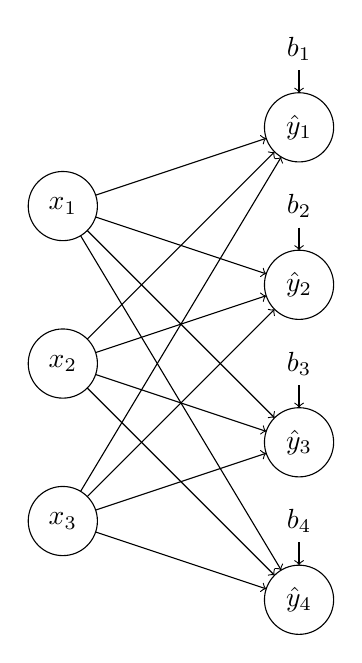
\begin{tikzpicture}
            [
                neuron/.style = {draw, circle, minimum size=25pt, inner sep=0pt, outer sep=0pt},
            ]
            \node [neuron] (x1) at (0,0) {$x_1$};
            \node [neuron] (x2) at (0,-2) {$x_2$};
            \node [neuron] (x3) at (0,-4) {$x_3$};
            \node [neuron] (n1) at (3,1)  {$\hat{y}_1$};
            \node [neuron] (n2) at (3,-1) {$\hat{y}_2$};
            \node [neuron] (n3) at (3,-3) {$\hat{y}_3$};
            \node [neuron] (n4) at (3,-5) {$\hat{y}_4$};
            \node (b1) at (3, 2) {$b_1$};
            \node (b2) at (3, 0) {$b_2$};
            \node (b3) at (3, -2) {$b_3$};
            \node (b4) at (3, -4) {$b_4$};
            \draw[->] (x1) -- (n1);
            \draw[->] (x1) -- (n2);
            \draw[->] (x1) -- (n3);
            \draw[->] (x1) -- (n4);
            \draw[->] (x2) -- (n1);
            \draw[->] (x2) -- (n2);
            \draw[->] (x2) -- (n3);
            \draw[->] (x2) -- (n4);
            \draw[->] (x3) -- (n1);
            \draw[->] (x3) -- (n2);
            \draw[->] (x3) -- (n3);
            \draw[->] (x3) -- (n4);
            \draw[->] (b1) -- (n1);
            \draw[->] (b2) -- (n2);
            \draw[->] (b3) -- (n3);
            \draw[->] (b4) -- (n4);
        \end{tikzpicture}
    \end{center}
    \caption{A single-layer perceptron with three input and four output neurons.}
    \label{fig:single_layer_perceptron}
\end{figure}

We purposefully use the term SLN instead of single-layer perceptron (SLP) to avoid confusion. 
A SLP has only one output unit and uses the threshold activation function given in (\ref{eq:thres_activation}) \cite{rosenblatt1958}.
In our definition of a SLN we allow more than one output and impose no restrictions on $g$, except that the same activation function is used for every output neuron.
We still use the term `single layer' because the input layer, lacking any incoming weight or bias connections, is not considered to be a `proper' layer.

Let us consider a SLN with $m$ inputs and $n$ outputs. 
Since every output unit $i$ only has connections from every input unit $j$,
we can adapt (\ref{eq:ann_activation}) to give the activation of a particular output neuron $i$ as
\begin{equation}
    a_i = y_i = g\left(z_i\right) = g\left(\sum_{j=1}^m{w_{j,i} x_j} + b_i\right)
    = g\left( \vec{w}_i\tran \vec{x}_i + b_i\right)
\end{equation}
where
$
    \vec{w}_i = \begin{bmatrix}
        w_{1,i} & w_{2,i} & \cdots & w_{m,i}
    \end{bmatrix}\tran
$
represents the weights of all the edges that connect to output unit $i$.
This is all we need to formally define a SLN.

\begin{definition}[Single-layer network]
    \label{def:sln}
    A SLN with $m$ inputs and $m$ outputs is the vector-valued function
    $\vec{S}: \mathbb{R}^m \rightarrow \mathbb{R}^n$ defined as
    \begin{equation}
        \label{eq:single_layer_perceptron}
        \vec{S}(\vec{x}; \vec{W}, \vec{b}) = \vec{g}\left( \vec{W}\tran \vec{x} + \vec{b} \right)
    \end{equation}
    where the  $m \times n$ matrix
    \begin{equation}
        \label{eq:sln_weight_matrix}
        \vec{W} = \begin{bmatrix}
            \vec{w}_1 & \vec{w}_2 & \cdots & \vec{w}_n
        \end{bmatrix} = \begin{bmatrix}
            w_{1,1} & w_{1,2} & \cdots & w_{1,n} \\
            w_{2,1} & w_{2,2} & \cdots & w_{2,n} \\
            \vdots & \vdots & \ddots & \vdots \\
            w_{m,1} & w_{m,2} & \cdots & w_{m,n}
        \end{bmatrix}
    \end{equation}
    captures all weights and the vector
    \begin{equation}
        \label{eq:sln_bias}
        \vec{b} = \begin{bmatrix}
            b_1 & b_2 & \cdots & b_n
        \end{bmatrix}\tran
    \end{equation}
    represents the biases.
    The vector-valued activation function $\vec{g} : \mathbb{R}^n \rightarrow \mathbb{R}^n$ is simply the activation function $g: \mathbb{R} \rightarrow \mathbb{R}$ applied pointwise to a vector, i.e.
    \begin{equation*}
        \vec{g}(\vec{z}) = \begin{bmatrix}
            g(z_1) & g(z_2) & \cdots & g(z_n)
        \end{bmatrix}\tran
    \end{equation*}
    for the vector of excitations
    $
        \vec{z} = \begin{bmatrix}
            z_1 & z_2 & \cdots & z_n
        \end{bmatrix}\tran
    $.
\end{definition}

Unlike the formula for a regression model, a SLN is a vector-valued function, due to the fact that there are multiple outputs. 
Note that when $n=1$, we reach the same form as in (\ref{eq:reg_model}). 
Moreover, if we additionally use the threshold activation function from (\ref{eq:thres_activation}), we arrive at the SLP model given by \textcite{rosenblatt1958}.

\subsection{Multi-layer perceptron}
\label{sec:multi_layer_perceptron}
A multi-layer perceptron\footnote{Unlike SLPs, the activation function in a MLP as defined in literature does not necessarily need to be the binary threshold function $g_\text{thres}$; in fact, it is often one of the more modern activation functions explained in Section \ref{sec:ann} \cite{hastie2017,burkov2019}. Hence we can use the term `multi-layer perceptron'.} (MLP) is a fully-connected feedforward ANN architecture with multiple layers which we will define in terms of multiple nested functions as in \textcite{burkov2019}.
\begin{definition}[Multi-layer perceptron]
    \label{def:mlp}
    A MLP $M$ with $m$ inputs and $L$ layers is the mathematical function
    $M : \mathbb{R}^m \rightarrow \mathbb{R}$ defined as the nested function
    \begin{equation}
        M(\vec{x}; \mathscr{P})
            = \hat{y}
            = f_L \left(
                \vec{f}_{L-1} \left(
                    \vec{\dots} \left(
                        \vec{f}_1 \left(
                            \vec{x}
                        \right)
                    \right)
                \right)
            \right)
    \end{equation}
    for the trainable parameters $\mathscr{P}=\langle\mathscr{W},\mathscr{B}\rangle$
    consisting of the weight matrices
    $\mathscr{W} = \vec{W}_1, \vec{W}_2, \dots, \vec{W}_L$
    and bias vectors
    $\mathscr{B} = \vec{b}_1, \vec{b}_2, \dots, \vec{b}_L$
    such that the nested functions are given by $\vec{f}_l(\vec{x}) = \vec{S}(\vec{x}; \vec{W}_l, \vec{b}_l)$ for $l = 1, \dots, L-1$.
    The outermost function $f_L$ represents a SLN with only one output unit and is hence the scalar-valued function $f_L(\vec{x}) = S(\vec{x}; \vec{W}_L, \vec{b}_L)$.
\end{definition}

Notice that for every $l < L$, $\vec{W}_l$ is a $n_l \times m_l$ matrix such that $n_l=m_{l+1}$ to esnure that the number of outputs of layer $l$ is the number of inputs to layer $l+1$.
This means that the MLP has $m_1$ input neurons.
Since the final layer has only one output unit, $\vec{W}_L$ has only one row, and finally $n_L=1$

The graph representing this type of network consists of connecting the outputs of the SLN representing layer $l$ with the inputs of the SLN representing layer $l+1$, as shown in Figure \ref{fig:multi_layer_perceptron}. 
The layers between the input and output layers are referred to as \textit{hidden} layers.

\begin{figure}
    \begin{center}
        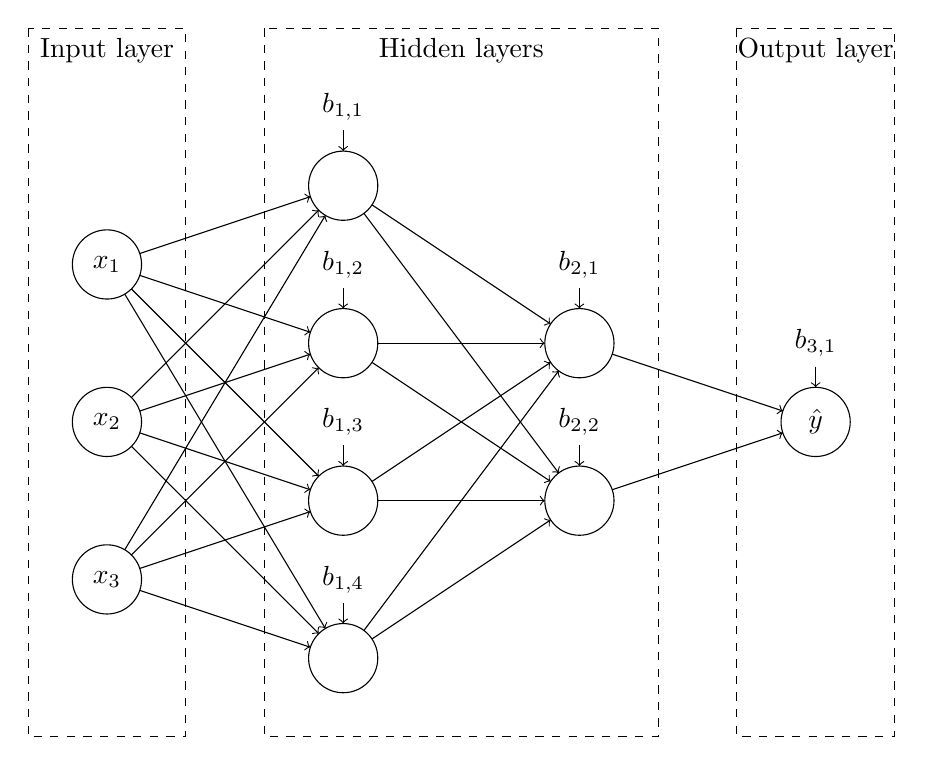
\begin{tikzpicture}
            [
                neuron/.style = {draw, circle, minimum size=25pt, inner sep=0pt, outer sep=0pt},
            ]
            \node [neuron] (x1) at (0,0) {$x_1$};
            \node [neuron] (x2) at (0,-2) {$x_2$};
            \node [neuron] (x3) at (0,-4) {$x_3$};
            \node [neuron] (h11) at (3,1) {};
            \node [neuron] (h12) at (3,-1) {};
            \node [neuron] (h13) at (3,-3) {};
            \node [neuron] (h14) at (3,-5) {};
            \node [neuron] (h21) at (6,-1) {};
            \node [neuron] (h22) at (6,-3) {};
            \node [neuron] (y) at (9, -2) {$\hat{y}$};
            \node (b11) at (3, 2) {$b_{1,1}$};
            \node (b12) at (3, 0) {$b_{1,2}$};
            \node (b13) at (3, -2) {$b_{1,3}$};
            \node (b14) at (3, -4) {$b_{1,4}$};
            \node (b21) at (6, 0) {$b_{2,1}$};
            \node (b22) at (6, -2) {$b_{2,2}$};
            \node (b3) at (9, -1) {$b_{3,1}$};
            \draw[->] (x1) -- (h11);
            \draw[->] (x1) -- (h12);
            \draw[->] (x1) -- (h13);
            \draw[->] (x1) -- (h14);
            \draw[->] (x2) -- (h11);
            \draw[->] (x2) -- (h12);
            \draw[->] (x2) -- (h13);
            \draw[->] (x2) -- (h14);
            \draw[->] (x3) -- (h11);
            \draw[->] (x3) -- (h12);
            \draw[->] (x3) -- (h13);
            \draw[->] (x3) -- (h14);
            \draw[->] (h11) -- (h21);
            \draw[->] (h11) -- (h22);
            \draw[->] (h12) -- (h21);
            \draw[->] (h12) -- (h22);
            \draw[->] (h13) -- (h21);
            \draw[->] (h13) -- (h22);
            \draw[->] (h14) -- (h21);
            \draw[->] (h14) -- (h22);
            \draw[->] (b11) -- (h11);
            \draw[->] (b12) -- (h12);
            \draw[->] (b13) -- (h13);
            \draw[->] (b14) -- (h14);
            \draw[->] (b21) -- (h21);
            \draw[->] (b22) -- (h22);
            \draw[->] (b3) -- (y);
            \draw[->] (h21) -- (y);
            \draw[->] (h22) -- (y);
            \draw[dashed] (-1,3) rectangle (1,-6);
            \draw[dashed] (2,3) rectangle (7,-6);
            \draw[dashed] (8,3) rectangle (10,-6);
            \node[below] (input) at (0,3) {Input layer};
            \node[below] (hidden) at (4.5,3) {Hidden layers};
            \node[below] (output) at (9,3) {Output layer};
        \end{tikzpicture}
    \end{center}
    \caption{A multi-layer perceptron with three inputs and two hidden layers.}
    \label{fig:multi_layer_perceptron}
\end{figure}

Since MLPs are simply nested SLNs, it follows that MLPs retain the DAG property and are therefore \textit{feedforward} networks as well.
In the forward pass, the activations are propagated from layer to layer (i.e. nested function to nested function) as in (\ref{eq:single_layer_perceptron}).

\section{The decision boundary in input space}
We will briefly introduce the concept of binary classification and show how it fits in the framework of the already defined regression model.
This will allow us to examine the so-called decision boundary in input space which will be useful for formulating the stripe problem (Section \ref{sec:stripe_problem}).

\begin{definition}[Binary classification model]
    A binary classification model $C$ is defined as a mathematical function of the form
    \begin{equation}
        C(\vec{x}) = \hat{y} = y + \epsilon
    \end{equation}
    with the same notation as in Definition \ref{def:reg_model} except that we impose the additional restriction that $y,\hat{y}\in \left\{0,1 \right\}$ such that the signature of the function becomes $C:\mathbb{R}^D\rightarrow \left\{0,1\right\}$.
\end{definition}
\begin{definition}[Decision boundary]
    Given a binary classification model $C$, the decision boundary is the hypersurface\footnote{A hypersurface is a manifold with one fewer dimension. Since the input space is $D$-dimensional, the hypersurface representing the decision boundary will have $D-1$ dimensions.} in input space $\mathcal{I}_C$ that separates the two output classes \cite[p. 723]{russell2010}.
    We will also use the term `hyperplane' to loosely refer to the decision boundary if it is flat/linear.
\end{definition}

\begin{lemma}
    Given a decision threshold $t$, we can use a regression model $R$ to solve any binary classification problem.
\end{lemma}
\begin{proof}
    We are looking define an equivalent classification model $C$ that outputs $0$ if $R\left(\vec{x}\right)<t$ and $1$ otherwise. 
    This can be achieved using the threshold activation function $g_\text{thres}$ from (\ref{eq:thres_activation}) in the form
    \begin{equation}
        C(\vec{x}) = g_\text{thres}\left(R\left(\vec{x}\right) - t\right).
    \end{equation}
\end{proof}
\begin{remark}
    What we have shown is that we can repurpose any regression model for a binary classification task, including for example MLPs.
    When using a MLP, the sigmoid activation function (\ref{eq:sigmoid}) naturally lends itself to be used on the output unit because its range, the interval $(0,1)$, can be interpreted as a probability.
    In this case we would set the decision threshold $t=\frac{1}{2}$.
\end{remark}

\begin{lemma}[Single-layer sigmoidal decision boundary]
    \label{lmm:sigmoid_decision_boundary}
    A single-layer sigmoidal MLP with a decision threshold $t \in (0,1)$ will have only one hyperplane in input space.
\end{lemma}
\begin{proof}
    Consider a single-layer MLP $M$ with $m$ inputs. 
    By Definition \ref{def:mlp}, this is equivalent to SLN $S$ with $m$ inputs and one output as shown in Figure \ref{fig:sln_m_in_1_out}. 
    \begin{figure}
        \begin{center}
            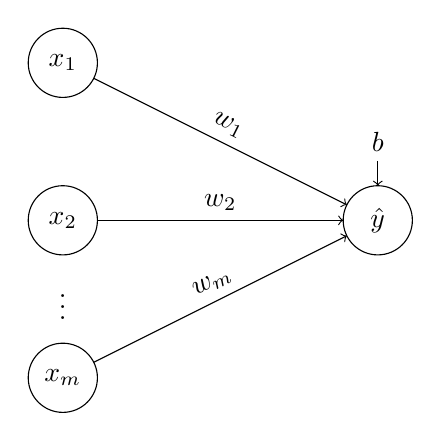
\begin{tikzpicture}
                [
                    neuron/.style = {draw, circle, minimum size=25pt, inner sep=0pt, outer sep=0pt},
                ]
                \node [neuron] (x1)  at (0,0) {$x_1$};
                \node [neuron] (x2) at (0,-2) {$x_2$};
                \node (dots) at (0,-3) {$\vdots$};
                \node [neuron] (xm) at (0,-4) {$x_m$};
                \node [neuron] (y) at (4,-2) {$\hat{y}$};
                \node (b) at (4, -1) {$b$};
                \draw[->] (x1) -- (y) node[midway, above, sloped] {$w_1$};
                \draw[->] (x2) -- (y) node[midway, above, sloped] {$w_2$};
                \draw[->] (xm) -- (y) node[midway, above, sloped] {$w_m$};
                \draw[->] (b) -- (y);
            \end{tikzpicture}
        \end{center}
        \caption{The DAG representing a SLN with $m$ inputs and one output unit.}
        \label{fig:sln_m_in_1_out}
    \end{figure}
    The equation of decision boundary can be obtained by setting the output equal to the decision threshold, so
    $t = S\left(\vec{x}\right)$
    for the input feature vector
    $\vec{x}= \begin{bmatrix}
        x_1 & x_2 & \cdots & x_m
    \end{bmatrix}\tran$.
    We have
    \begin{align*}
        t &= S\left(\vec{x}\right) \\
        &= g_\text{sig}\left(\vec{w}\tran \vec{x} + b\right) \\
        &= \frac{1}{1+e^{-\vec{w}\tran \vec{x} - b}} \\
        \frac{1}{t} - 1 &= e^{-\vec{w}\tran \vec{x} - b} \\
        \ln \left(\frac{1}{t} - 1\right) &= -\vec{w}\tran \vec{x} - b.
    \end{align*}
    For $\ln \left(\frac{1}{t} - 1\right)$ to be real-valued, we must ensure that $\frac{1}{t} - 1 > 0$ which is the case because $0<t<1$.

    We obtain only one linear equation of the form
    \begin{equation}
        \label{eq:sigmoid_hyperplane}
        0=w_1 x_2 + w_2 x_2 + \dots + w_m x_m + b + \ln \left(\frac{1}{t} - 1\right)
    \end{equation}
    which means that there is only one hyperplane.
\end{proof}

\begin{example}
    \label{ex:sln_2_in_1_out_sigmoid_hyperplane}
    Let us consider a MLP $M$ with only one layer and two inputs, as depicted in Figure \ref{fig:sln_2_in_1_out}.
    \begin{figure}
        \begin{center}
            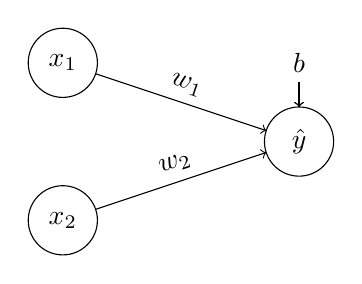
\begin{tikzpicture}
                [
                    neuron/.style = {draw, circle, minimum size=25pt, inner sep=0pt, outer sep=0pt},
                ]
                \node [neuron] (x1) at (0,0) {$x_1$};
                \node [neuron] (x2) at (0,-2) {$x_2$};
                \node [neuron] (y) at (3,-1)  {$\hat{y}$};
                \node (b) at (3, 0) {$b$};
                \draw[->] (x1) -- (y) node[above,midway,sloped] {$w_1$};
                \draw[->] (x2) -- (y) node[above,midway,sloped] {$w_2$};
                \draw[->] (b) -- (y);
                \draw[->] (b) -- (y);
            \end{tikzpicture}
        \end{center}
        \caption{A simple MLP with one layer and two inputs (equivalently, a SLN with two inputs and one ouput).}
        \label{fig:sln_2_in_1_out}
    \end{figure}
    We will consider the configuration where $w_1=w_2=1$ and $b=0$. 
    The output unit will have the sigmoid activation function, and we will choose the decision threshold $t=\frac{1}{2}$.
    
    The decision boundary will be a line because $\mathcal{I}_M$ has two dimensions, and a hyperplane in a two-dimensional space is simply a line.
    The equation of this line can be obtained from (\ref{eq:sigmoid_hyperplane}) as
    \begin{align*}
        0 &= w_1 x_1 + w_2 x_2 + b + \ln \left(\frac{1}{\left(\frac{1}{2}\right)} - 1\right) \\
        &= x_1 + x_2 + \ln 1 \\
        x_2 &= -x_1.
    \end{align*}

    Figure \ref{fig:sigmoid_hyperplane} depicts this hyperplane along with some samples in input space to show how they would be classified. 
    The arrow on the hyperplane shows the direction of increasing output, i.e. what would be classified as $1$.
    \begin{figure}
        \centering
        \begin{tikzpicture}
            \begin{axis}[
                x=1cm,
                y=1cm,
                axis lines=center,
                xlabel={$x_1$}, xlabel style={anchor=west},
                ylabel={$x_2$}, ylabel style={anchor=south},
                ymin=-3.2, ymax=3.2,
                xmin=-3.2, xmax=3.2,
                samples=2
            ]
                \addplot[black,only marks,mark=*] coordinates {(1,1) (-2,3) (2,0) (3,-2) (2,3) (-1,2) (3,1)};
                \addplot[black,only marks,mark=o] coordinates {(-1,-1) (2,-3) (-2,0) (-3,2) (-2,-3) (1,-2) (-3,-1)};
                \addplot[black, no marks] {-x};
                \addplot[black, ->] coordinates {(-2, 2) (-1.5, 2.5)};
            \end{axis}
        \end{tikzpicture}
        \caption{Plot of the input space of the MLP from Figure \ref{fig:sln_2_in_1_out} with sigmoid activation where $w_1=w_2=1$, $b=0$, and some sample data. Filled in dots represent a prediction of $\hat{y}>\frac{1}{2}$ whereas the empty circular dots represent $\hat{y}<\frac{1}{2}$.}
        \label{fig:sigmoid_hyperplane}
    \end{figure}
\end{example}

\chapter{Neural network training}
This chapter will introduce two methods of training neural networks to provide an intuition on how this can be achieved.
Later in this report, we will look at some issues related to these methods as a means of setting the scene for the neural surfing technique.

In this context, \textit{training} refers to the process of changing the network's weights and biases with the goal of achieving an optimal configuration that reduces the error of the predictions, i.e. how far they are `off'. 
We will use a simple loss function that uses mean squared error for this purpose.
\begin{definition}[Mean squared error]
    Let $\left\{\langle \vec{x}_i, y_i \rangle \right\}_{i=1}^N$ be a labelled dataset (see Definition \ref{def:labelled_dataset}).
    The mean squared error of a set of predictions $\vec{\hat{y}}$ is given as an average over the sum of squared differences,
    \begin{equation}
        \label{eq:mean_squared_error}
        E\left( \vec{y}, \vec{\hat{y}} \right) = \frac{1}{N} \sum_{i=1}^N{\left(\hat{y}_i - y_i\right)^2}.
    \end{equation}
\end{definition}

\begin{definition}[Loss function]
    Given an MLP $M$ with $P$ trainable parameters (weights and biases), the loss function $L:\mathbb{R}^P\rightarrow \mathbb{R}$ is a function that maps weight (and bias) configurations to their associated error values.
    Let $\vec{y} \in \mathbb{R}^N$ be the target outputs for training.
    Then the loss function is defined as
    \begin{equation}
        L(\vec{p}) = \sum_{i=1}^N{\left(M\left(\vec{x}_i; \vec{p}\right) - y_i\right)^2}.
    \end{equation}
    Notice the similarity to (\ref{eq:mean_squared_error}). 
    However, we have omitted the factor $\frac{1}{N}$ since the actual loss values are not as important as their relationship to each other, and multiplying by $N$ will retain that relationship.
    We use the term \textit{error-weight surface} to refer to the graph of this function.
\end{definition}

\section{Backpropagation}
Backpropagation (BP) via gradient descent is an iterative algorithm for training neural networks that, provided a suitable learning rate $\alpha$, is guaranteed to converge to a \textit{local minimum} (see Section \ref{sec:local_minimum_problem}).
The main idea is as follows:
\begin{enumerate}
    \item Calculate the derivative of the loss function with respect to the current trainable parameters $\vec{p}$ as
        $\vec{\Delta p} = \frac{\delta L}{\delta \vec{p}}\left(\vec{p}\right)$.
    \item Take a step in the negative direction of this gradient, i.e. update the trainable parameters $\vec{p} \leftarrow \vec{p} - \alpha \vec{\Delta p}$ where $\alpha \in \mathbb{R}$ is the learning rate.
    \item Repeat steps 1 and 2 until a predefined convergence criterion is met.
\end{enumerate}
Figure \ref{fig:gradient_descent_local_minimum} shows the steps that this algorithm would make on a simple error-weight surface with only one parameter.
\begin{figure}
    \centering
    \begin{tikzpicture}[
        declare function={
            f(\x) = \x^4 + 0.5*\x^3 - 2*\x^2;
            g(\x) = f(.5*\x-2)+2;
        }
    ]
        \begin{axis}[
            x=1.5cm,
            y=1.5cm,
            axis lines=center,
            xlabel={$p$}, xlabel style={anchor=west},
            ylabel={$L(p)$}, ylabel style={anchor=south},
            ymin=-0, ymax=4.2,
            xmin=0, xmax=7.2,
            samples=50,
            domain=0.1:7.5,
            ticks=none
        ]
            \addplot[black] {g(x)};
            \addplot[-{Latex[length=2mm]},black,samples at={6.85,6.5},mark=*] {g(x)};
            \addplot[-{Latex[length=2mm]},black,samples at={6.5,6.2},mark=*] {g(x)};
            \addplot[-{Latex[length=2mm]},black,samples at={6.2,5.9},mark=*] {g(x)};
            \addplot[-{Latex[length=2mm]},black,samples at={5.9,5.7},mark=*] {g(x)};
            \node[left] at (6.85,{g(6.85)}) {initial position};
            \node[below,align=center] at (5.7,{g(5.7)}) {final position\\(local minimum)};
            \addplot[mark=*] coordinates {(1.6,{g(1.6)})};
            \node[below,align=center] at (1.6,{g(1.6)}) {global minimum};
        \end{axis}
    \end{tikzpicture}
    \caption{An illustration gradient descent training on an error-weight surface with only one parameter (not drawn to scale).}
    \label{fig:gradient_descent_local_minimum}
\end{figure}

Calculating the derivative of the loss function with respect to each of the trainable parameters is a core part of the gradient descent algorithm.
Let us look at calculating this gradient for the example of a single-layer MLP. 
We will come back to these results in Section \ref{sec:stripe_problem}.
\begin{example}[Gradient in a single-layer MLP]
    Let us revisit the SLN with $m$ inputs and one output from Figure \ref{fig:sln_m_in_1_out}.
    The loss function will be in terms of the trainable parameters, i.e. the weights $\vec{w}$ and bias $b$, so
    \begin{align}
        L = L(\vec{w}, b)
        &= \sum_{i=1}^N{\left(S\left(\vec{x}_i; \vec{w}, b\right) - y_i\right)^2} \nonumber \\
        &= \sum_{i=1}^N{\left(g\left(\vec{w}\tran \vec{x}_i + b\right) - y_i\right)^2}.
    \end{align}

    We obtain the partial derivative of the loss with respect to the bias as
    \begin{align}
        \frac{\delta L}{\delta b}
        &=2 \sum_{i=1}^N{
            \left(g \left(\vec{w}\tran\vec{x}_i+b\right) - y_i \right)
            \frac{\delta}{\delta b} \left(g \left(\vec{w}\tran\vec{x}_i+b\right) - y_i \right)
        } \nonumber \\
        &= 2 \sum_{i=1}^N{
            \left(g \left(\vec{w}\tran\vec{x}_i+b\right) - y_i \right)
            g' \left(\vec{w}\tran\vec{x}_i+b\right)
        },
    \end{align}
    and similarly we can differentiate with respect to the weights
    \begin{align}
        \frac{\delta L}{\delta \vec{w}}
        &= 2 \sum_{i=1}^N{
            \left(g \left(\vec{w}\tran\vec{x}_i+b\right) - y_i \right)
            \frac{\delta}{\delta \vec{w}} \left(g \left(\vec{w}\tran\vec{x}_i+b\right) - y_i \right)
        } \nonumber \\
        &= 2 \sum_{i=1}^N{
            \left(g \left(\vec{w}\tran\vec{x}_i+b\right) - y_i \right)
            g' \left(\vec{w}\tran\vec{x}_i+b\right)
            \vec{x}_i
        }.
    \end{align}

    Now we would denote the gradient of the loss with respect to the trainable parameters $\vec{p}$ as the row vector
    \begin{equation*}
        \frac{\delta L}{\delta \vec{p}} = \begin{bmatrix}
            \frac{\delta L}{\delta w_1} &
            \frac{\delta L}{\delta w_2} &
            \cdots &
            \frac{\delta L}{\delta w_m} &
            \frac{\delta L}{\delta b}
        \end{bmatrix}.
    \end{equation*}
\end{example}


\section{Greedy probing}
Unlike BP, greedy probing is a simple derivative-free optimisation (DFO) technique. 
At each iteration, the algorithm will sample a predefined number of configurations in the local neighbourhood of the current parameter configuration $\vec{p}$. 
The loss is calculated at each of these samples, and the best (i.e. lowest value) is chosen as the new parameter configuration. 
In this sense, greedy probing is similar to gradient descent, except that the gradient is manually calculated instead of using the partial derivative.
As a result, greedy probing will suffer similar issues as gradient descent, but depending on the sampling radius $r \in \mathbb{R}$ it is conjectured that it might be less sensitive to local pertubations (`noise') on the error-weight surface.

The sampling technique may either be \textit{exhaustive} or \textit{random}.
In the exhaustive case, the samples around point $\vec{p}_i$ are given by
\begin{equation}
    \left\{
        \vec{p}_i + r
        \frac{
            \begin{bmatrix}
                p_1 & p_2 & \cdots & p_P
            \end{bmatrix}\tran
        }{
            \norm{
                \begin{bmatrix}
                    p_1 & p_2 & \cdots & p_P
                \end{bmatrix}
            }
        }
        : \begin{array}{l}
            \text{$p_1, p_2, \dots, p_P \in \left\{-1,0,1\right\}$ and} \\
            \norm{
                \begin{bmatrix}
                    p_1 & p_2 & \cdots & p_P
                \end{bmatrix}
            } \neq 0
        \end{array}
    \right\}
\end{equation}
which means that $3^P-1$ samples are generated at each iteration.
On the other hand, the random sampling technique will generate a predefined number of random samples in weight space with the condition that given the current configuration $\vec{p}_i$, for every candidate sample $\vec{\hat{p}}$, it must be true that
$\norm{\vec{p}_i - \vec{\hat{p}}} = r$.


\section{Simulated annealing}
The rationale of the simulated annealing (SA) algorithm lies in its analogy to the behaviour that atoms exhibit in a substance that is slowly cooling down \cite{kirkpatrick1983}.
At high temperatures, the atoms move around with high kinetic energy, but as the temperature cools down, they begin to move more slowly until completely losing thermal mobility. 
When this process is carried out sufficiently slowly, the atoms will settle in a perfectly aligned crystal structure with minimum energy. 
However, if the cooling process is too fast, the final structure will be chaotic and hence not be at the minimum energy state \cite[p. 444]{press1992}.

At each iteration, the algorithm will explore random sample points one after another in the local neighbourhood of the current configuration $\vec{p}_i$ until one is accepted. 
The probability of accepting a candidate sample point $\vec{\hat{p}}$ at the $i$th iteration is given by the probability distribution
\begin{equation}
    P(\vec{\hat{p}}|\vec{p}_i) = \begin{cases}
        \exp{\left(-\frac{k}{T_i} \left(L(\vec{\hat{p}}) - L(\vec{p}_i)\right) \right)} & L(\vec{\hat{p}}) > L(\vec{p}_i) \\
        1 & L(\vec{\hat{p}}) \leq L(\vec{p}_i)
    \end{cases}
\end{equation}
for an energy coefficient $k\in \mathbb{R}$ \cite{rios2009}.
This means that the SA algorithm will always accept a better location, but, with a certain probability, might take a suboptimal step.

The temperature at the $i$ iteration is determined according to a \textit{cooling schedule}. 
We will employ a simple approach as a proof of concept that calculates $T_i$ as the geometric sequence
\begin{equation}
    T_i = \left(1 - c\right) T_{i-1} = \left(1 - c\right)^i T_0
\end{equation}
where $c$ is a cooling rate typically of the order of $10^{-1}$ or $10^{-2}$.
Already, this simple SA algorithm has three hyperparameters: the energy coefficient $k$, the initial temperature $T_0$, and the cooling rate $c$. 
More sophisticated implementations will require even more hyperparameters (such as \textcite{press1992} as remarked in Section \ref{sec:eval_sim_annealing}) that makes it increasingly difficult to design SA in a generic fashion to suit the training of neural networks. 


\chapter{The local minimum problem}
\label{sec:local_minimum_problem}

\section{The mathematics of local and global minima}

\begin{definition}[Global minimum]
    The function $f: \mathbb{R}^n \rightarrow \mathbb{R}$ has a \textit{global minimum} at point
    $\vec{p} \in \mathbb{R}^n$
    if and only if for all
    $\vec{x} \in \mathbb{R}^n$
    it is true that
    $f(\vec{p}) \leq f(\vec{x})$.
\end{definition}

\begin{definition}[Local minimum]
    \label{def:local_minimum}
    The function $f: \mathbb{R}^n \rightarrow \mathbb{R}$ has a \textit{local minimum} at point
    $\vec{p} \in \mathbb{R}^n$
    if there exists a ball with centre
    $\vec{p}$
    where
    $f(\vec{p}) \leq f(\vec{x})$
    for all points $\vec{x}$ in that ball.
    A \textit{suboptimal local minimum} is a local minimum that is not a global minimum.
\end{definition}

\begin{definition}[Jacobian]
    Let $f: \mathbb{R}^n \rightarrow \mathbb{R}$ be a continuously differentiable function of the form
    $f=f\left(\vec{x}\right)$
    where
    $\vec{x} = \begin{bmatrix}
        x_1 & x_2 & \cdots & x_n
    \end{bmatrix}\tran$.
    The Jacobian of $f$ (or simply \textit{derivative} of $f$) is a row vector of its first-order partial derivatives,
    \begin{equation*}
        \vec{J}_f
        = \frac{\delta f}{\delta \vec{x}}
        = \begin{bmatrix}
            \frac{\delta f}{\delta x_1} &
            \frac{\delta f}{\delta x_2} &
            \cdots &
            \frac{\delta f}{\delta x_n}
        \end{bmatrix}.
    \end{equation*}
\end{definition}
\begin{definition}[Hessian]
    Let $f: \mathbb{R}^n \rightarrow \mathbb{R}$ be a function of the form
    $f=f\left(\vec{x}\right)$
    where
    $\vec{x} = \begin{bmatrix}
        x_1 & x_2 & \cdots & x_n
    \end{bmatrix}\tran$
    for which all second partial derivatives exist and are continuous over $\mathbb{R}^n$.
    The Hessian of $f$ is a $n\times n$ matrix of the second-order partial derivatives, given by
    \begin{equation*}
        \vec{H}_f = \begin{bmatrix}
            \frac{\delta^2 f}{\delta x_1^2} &
            \frac{\delta^2 f}{\delta x_1 x_2} &
            \cdots &
            \frac{\delta^2 f}{\delta x_1 x_n} \\
            \frac{\delta^2 f}{\delta x_2 x_1} &
            \frac{\delta^2 f}{\delta x_2^2} &
            \cdots &
            \frac{\delta^2 f}{\delta x_2 x_n} \\
            \vdots & \vdots & \ddots & \vdots \\
            \frac{\delta^2 f}{\delta x_n x_1} &
            \frac{\delta^2 f}{\delta x_n x_2} &
            \cdots &
            \frac{\delta^2 f}{\delta x_n^2}
        \end{bmatrix}.
    \end{equation*}
\end{definition}
\begin{definition}[Positive definite matrix]
    \label{def:positive_definite}
    A symmetric $n\times n$ matrix $\vec{M} \in \mathbb{R}^{n\times n}$ is said to be \textit{positive definite} if and only if
    $\vec{x}\tran \vec{M} \vec{x} > 0$
    for all $\vec{x} \in \mathbb{R}^n \setminus \vec{0}$.
\end{definition}
We will prove a simple technique for showing that a $2 \times 2$ matrix is positive definite, as this will help us prove the existence of local minima later.
\begin{theorem}[$2\times 2$ positive definite matrix]
    \label{thm:positive_definite_2_by_2}
    The matrix $\vec{M} = \begin{bmatrix}
        a & b \\ b & c
    \end{bmatrix}$
    is positive definite if
    $a > 0$ and 
    $ac - b^2>0$.
\end{theorem}
\begin{proof}
    Let $\vec{x} = \begin{bmatrix}
        x_1 & x_2
    \end{bmatrix}\tran$
    and $f(x_1, x_2) = \vec{x}\tran \vec{M} \vec{x}$.
    Performing the multiplication,
    \begin{align*}
        f(x_1, x_2)
        &= 
        \begin{bmatrix}
            x_1 & x_2
        \end{bmatrix}
        \begin{bmatrix}
            a & b \\
            b & c
        \end{bmatrix}
        \begin{bmatrix}
            x_1 \\ x_2
        \end{bmatrix} \\
        &=
        \begin{bmatrix}
            x_1 a + x_2 b & x_1 b + x_2 c
        \end{bmatrix}
        \begin{bmatrix}
            x_1 \\ x_2
        \end{bmatrix} \\
        &=
            x_1^2 a + 2 x_1 x_2 b + x_2^2 c.
    \end{align*}

    We will now discuss under what conditions
    $f(x_1, x_2) > 0$
    holds.
    When $x_2=0$, it must necessarily be the case that $a>0$.
    Otherwise, dividing by $x_2^2$, we can write
    \begin{align*}
        \left(\frac{x_1}{x_2}\right)^2 a + \frac{2 x_1 b}{x_2} + c > 0,
    \end{align*}
    and substituting $p = \frac{x_1}{x_2}$ we get
    \begin{align*}
        p^2 a + 2pb + c > 0.
    \end{align*}
    Treating this as a quadratic function in terms of $p$, we realize that since $a>0$, the parabola opens up.
    The discriminant $D=4b^2 - 4ac$ is negative if $ac-b^2>0$ which means that the parabola has no roots. 
    Thus its range is positive.

    We have shown that $f(x_1, x_2)>0$ if $a>0$ and $ac-b^2>0$ for all $x_1,x_2\in \mathbb{R}$ except $x_1=x_2=0$.
    By Definition \ref{def:positive_definite}, $\vec{M}$ must be positive definite.
\end{proof}

\begin{theorem}[Local minimum]
    Let $f: \mathbb{R}^n \rightarrow \mathbb{R}$ be a continuously differentiable function, and let the point
    $\vec{p} \in \mathbb{R}^n$
    be such that
    $\vec{J}_f(\vec{p}) = \vec{0}$
    and
    $\vec{H}_f(\vec{p})$ is positive definite.
    Then $\vec{p}$ is a \textit{local minimum} of $f$.
\end{theorem}
We will require this theorem to prove that training converges to a local minimum in Section \ref{sec:stripe_problem}.
However, the proof of this theorem exceeds the scope of this report.
The interested reader may consult \textcite[p. 190]{loomis1990}.

\section{The suboptimal local minimum problem}
\todo: explain local minimum problem with respect to gradient descent, greedy probing, and SA (+ random initialisation)


\chapter{Neural surfing theory}

\section{Weight and output spaces}
In Definition \ref{def:mlp} we established that the tuple $\langle \mathscr{W}, \mathscr{B} \rangle$ along with the activation function is sufficient to fully define a MLP. 
Most importantly, we have $\mathscr{W} = \vec{W}_1, \vec{W}_2, \dots, \vec{W}_L$ and $\mathscr{B} = \vec{b}_1, \vec{b}_2, \dots, \vec{b}_L$ representing each layer's weight matrices and bias vectors, respectively. 
These parameters will be useful for defining the weight and ouput spaces.

\begin{definition}[Weight space]
    \label{def:weight_space}
    The weight space $\mathcal{W}_A$ of an artificial neural network $A$ is the set of all possible assignments to its \textit{trainable parameters}. 
    The trainable parameters are its weights $\mathscr{W}$ and biases $\mathscr{B}$.
    If $A$ has $P$ trainable parameters then its weight space is defined as
    \begin{equation}
        \mathcal{W}_A = \mathbb{R}^P.
    \end{equation}
\end{definition}

\begin{definition}[Output space]
    \label{def:output_space}
    The output space $\mathcal{O}_A$ of an artificial neural network $A$ with one output neuron spans the space of all possible output predictions on the training set.
    From (\ref{eq:sup_learn_prediction}), the vector $\vec{\hat{y}}$ represents the prediction $\hat{y}$ for all $N$ training samples.
    The output space spans all possible assignments of $\vec{\hat{y}}$, so
    \begin{equation}
        \mathcal{O_A}=\mathbb{R}^N.
    \end{equation}
\end{definition}

\begin{lemma}
    \label{lmm:weight_space_sln}
    The weight space for a SLN $S$ with $m$ inputs and $n$ outputs is $\mathcal{W}_S = \mathbb{R}^{n(m+1)}$.
\end{lemma}
\begin{proof}
    $S$'s trainable parameters are the weight matrix $\vec{W} \in \mathbb{R}^{m\times n}$ from (\ref{eq:sln_weight_matrix}) and bias vector $\vec{b} \in \mathbb{R}^n$ from (\ref{eq:sln_bias}).
    By Definition \ref{def:weight_space}, the weight space encompasses all values of $\vec{W}$ and $\vec{b}$, so
    \begin{equation*}
        \mathcal{W}_S = \mathbb{R}^{m \times n} \times \mathbb{R}^{n} = \mathbb{R}^{m n + n} = \mathbb{R}^{(m + 1) n}.
    \end{equation*}
\end{proof}

\begin{lemma}
    \label{lmm:weight_space_mlp}
    A MLP $M$ with $L$ layers where the number of inputs to layer $l$ is given as $m_l$ will have the weight space $\mathcal{W}_M = \mathbb{R}^P$ where
    $P = \sum_{l=1}^{L-1}{\left(m_{l+1} (m_l + 1)\right)} + m_L + 1$.
\end{lemma}

\begin{proof}
    By Definition \ref{def:mlp}, $M$ is comprised of $L$ SLNs which we will denote $\vec{S}_1, \vec{S}_2, \dots, S_L$.
    This allows us to express the weight space of $M$ as the product of the weight spaces of each of the SLNs,
    $$
        \mathcal{W}_M
        = \prod_{l=1}^L{\mathcal{W}_{S_l}}.
    $$

    For every layer $l$, the number of inputs to $S_l$ will be the number of inputs to the $l$th layer, $m_l$. 
    Let $n_l$ denote the number outputs for each layer $l$.
    Then, by Lemma \ref{lmm:weight_space_sln},
    $$\mathcal{W}_{S_l} = \mathbb{R}^{n_l(m_l+1)}.$$
    
    By splitting of the last factor in the product of weight spaces, we obtain 
    \begin{equation*}
        \mathcal{W}_M
        = \prod_{l=1}^{L-1}{\mathcal{W}_{S_l}} \times \mathcal{W}_{S_L}
        = \prod_{l=1}^{L-1}{\mathbb{R}^{n_l(m_l+1)}} \times \mathbb{R}^{n_L(m_L+1)}.
    \end{equation*}

    Notice that for any layer $l$, the number of outputs is equal to the number of inputs to the next layer, so $n_l=m_{l+1}$ except for the last layer where there is only one output unit leaving $n_L=1$.
    This leaves
    \begin{align*}
        \mathcal{W}_M
        &= \prod_{l=1}^{L-1}{\mathbb{R}^{m_{l+1}(m_l+1)}} \times \mathbb{R}^{m_L+1} \\
        &= \mathbb{R}^{\sum_{l=1}^{L-1}{m_{l+1}(m_l+1)}} \times \mathbb{R}^{m_L+1} \\
        &= \mathbb{R}^{\sum_{l=1}^{L-1}{m_{l+1}(m_l+1)} + m_L+1},
    \end{align*}
    so $\mathcal{W}_M = \mathbb{R}^P$ with
    \begin{equation*}
        P = \sum_{l=1}^{L-1}{m_{l+1}(m_l+1)} + m_L+1.
    \end{equation*}
\end{proof}

\begin{remark}
    The significance of Lemma \ref{lmm:weight_space_mlp} is that we obtain a formula for the number of trainable parameters $P$ in a MLP. 
    By Definition \ref{def:weight_space}, $P$ determines the dimensionality of the weight space. 
    On other other hand, Definition \ref{def:output_space} states that the number of samples in the training set $N$ determines the dimensionality of the output space.
    There is no relationship between $P$ and $N$ since the number of samples in the training set can be arbitrarily chosen. 
    It follows that there is no relationship between the dimensionalities of $\mathcal{W}$ and $\mathcal{O}$.
\end{remark}

\subsection{Relationship between weight and output space}
We will now examine the nature of the mapping between the two spaces, and whether there exists a linear mapping. 
Note that linear mappings can exist between spaces of different dimensionalities \cite{rudin2006}.

\begin{definition}[Weight-output mapping]
    \label{def:weight_output_space_mapping}
    Given an artifical neural network $A:\mathbb{R}^m \rightarrow \mathbb{R}^n$ with $m$ inputs and $n$ outputs parameterized by a set of trainable parameters $\vec{w} \in \mathcal{W_A}$,
    the weight-to-output-space mapping $h_A: \mathcal{W}_A \rightarrow \mathcal{O}_A$ for a dataset with $N$ $m$-dimensional feature vectors given by the matrix
    $\vec{X} = \begin{bmatrix}
        \vec{x}_1 & \vec{x}_2 & \cdots & \vec{x}_N
    \end{bmatrix}\tran \in \mathbb{R}^{N\times m}$
    is
    \begin{equation*}
        h_A \left( \vec{w} \right)
        = \begin{bmatrix}
            A(\vec{x}_1; \vec{w} ) \\
            A(\vec{x}_2; \vec{w} ) \\
            \vdots \\
            A(\vec{x}_N; \vec{w} ) \\
        \end{bmatrix}.
    \end{equation*}

    Note that we use the term `weight-output mapping' to refer to the `weight-to-output-space mapping' which should be confused with the mapping from weight space to a particular output prediction. 
\end{definition}

\begin{theorem}
    \label{thm:sln_one_output}
    For a SLN $S$ with one output unit, the function $h_S: \mathcal{W}_S \rightarrow \mathcal{O}_S$ is not a linear mapping.
\end{theorem}
\begin{proof}
    Let $S$ have $m$ inputs, as depicted in Figure \ref{fig:sln_m_in_1_out}.
    Modifying the formula for a SLN given in Definition \ref{def:sln} (\ref{eq:single_layer_perceptron}) for the case where there is only one output unit, we obtain
    $\hat{y} = f_\text{SLP}(\vec{x}; \vec{w}\tran, b) = g\left(\vec{w} \vec{x} + b\right)$
    where
    $\vec{x} = \begin{bmatrix}
        x_1 & x_2 & \cdots & x_m
    \end{bmatrix}\tran$
    is the input feature vector.

    We will consider a dataset with $N$ samples where the input is given by the $N\times m$ matrix
    $\vec{X} = \begin{bmatrix}
        \vec{x}_1 & \vec{x}_2 & \cdots & \vec{x}_N
    \end{bmatrix}\tran$
    as in (\ref{eq:sup_learn_input_matrix}).
    By Definition \ref{def:weight_output_space_mapping}, the mapping from weight to output space $h_S: \mathcal{W}_S \rightarrow \mathcal{O}_S$ is
    \begin{equation*}
        h_S \left( \vec{w} \right)
        = \begin{bmatrix}
            g \left( \vec{w}\tran \vec{x}_1 + b \right) \\
            g \left( \vec{w}\tran \vec{x}_2 + b \right) \\
            \vdots \\
            g \left( \vec{w}\tran \vec{x}_N + b \right) \\
        \end{bmatrix}.
    \end{equation*}

    We will assume, by way of contradiction, that $h$ is a linear mapping. 
    From the definition of linear mappings, it must be true that $h(\vec{u} + \vec{v}) = h(\vec{u}) + h(\vec{v})$ for $\vec{u}, \vec{v} \in \mathcal{W}_S$ \cite{rudin2006}.
    On the LHS we have
    \begin{equation*}
        h \left( \vec{u} + \vec{v} \right)
        = \begin{bmatrix}
            g((\vec{u} + \vec{v})\tran \vec{x}_1 + b) \\
            g((\vec{u} + \vec{v})\tran \vec{x}_2 + b) \\
            \vdots \\
            g((\vec{u} + \vec{v})\tran \vec{x}_N + b) \\
        \end{bmatrix}
        = \begin{bmatrix}
            g(\vec{u}\tran \vec{x}_1 + \vec{v}\tran \vec{x}_1 + b) \\
            g(\vec{u}\tran \vec{x}_2 + \vec{v}\tran \vec{x}_2 + b) \\
            \vdots \\
            g(\vec{u}\tran \vec{x}_N + \vec{v}\tran \vec{x}_N + b) \\
        \end{bmatrix}
    \end{equation*}
    and on the RHS we get
    \begin{equation*}
        h \left( \vec{u} \right) + h \left( \vec{v} \right)
        = \begin{bmatrix}
            g(\vec{u}\tran \vec{x}_1 + b) \\
            g(\vec{u}\tran \vec{x}_2 + b) \\
            \vdots \\
            g(\vec{u}\tran \vec{x}_N + b) \\
        \end{bmatrix}
        + \begin{bmatrix}
            g(\vec{v}\tran \vec{x}_1 + b) \\
            g(\vec{v}\tran \vec{x}_2 + b) \\
            \vdots \\
            g(\vec{v}\tran \vec{x}_N + b) \\
        \end{bmatrix}
        = \begin{bmatrix}
            g(\vec{u}\tran \vec{x}_1 + b) + g(\vec{v}\tran \vec{x}_1 + b) \\
            g(\vec{u}\tran \vec{x}_2 + b) + g(\vec{v}\tran \vec{x}_2 + b) \\
            \vdots \\
            g(\vec{u}\tran \vec{x}_N + b) + g(\vec{v}\tran \vec{x}_N + b) \\
        \end{bmatrix},
    \end{equation*}
    leaving
    \begin{equation*}
        \begin{bmatrix}
            g(\vec{u}\tran \vec{x}_1 + \vec{v}\tran \vec{x}_1 + b) \\
            g(\vec{u}\tran \vec{x}_2 + \vec{v}\tran \vec{x}_2 + b) \\
            \vdots \\
            g(\vec{u}\tran \vec{x}_N + \vec{v}\tran \vec{x}_N + b) \\
        \end{bmatrix}
        = \begin{bmatrix}
            g(\vec{u}\tran \vec{x}_1 + b) + g(\vec{v}\tran \vec{x}_1 + b) \\
            g(\vec{u}\tran \vec{x}_2 + b) + g(\vec{v}\tran \vec{x}_2 + b) \\
            \vdots \\
            g(\vec{u}\tran \vec{x}_N + b) + g(\vec{v}\tran \vec{x}_N + b) \\
        \end{bmatrix}.
    \end{equation*}

    Let $\alpha_i = \vec{u}\tran \vec{x}_i$ and $\beta_i = \vec{v}\tran \vec{x}_i$ for all $i$.
    Since $\vec{u},\vec{v} \in \mathbb{R}^m$ and all $\vec{x}_i \in \mathbb{R}^m$, it follows that $\alpha_i, \beta_i \in \mathbb{R}$ for all $i$.
    Hence $g(\alpha + \beta + b) = g(\alpha + b) + g(\beta + b)$.

    The only functions that satisfy $g$ are functions that satisfy Cauchy's functional equation\footnote{Cauchy's functional equation is $f(a+b)=f(a)+f(b)$. For $a,b \in \mathbb{Q}$, the only solutions are linear functions of the form $f(x) = cx$ for some $c \in \mathbb{Q}$ \cite{reem2017}.}, but these solutions only apply when $b=0$ and furthermore are linear, whereas the activation function $g$ is non-linear. 
    We arrived at a contradiction, thus disproving our initial assumption that $h$ is a linear mapping, so it must be a non-linear mapping.
\end{proof}

\begin{corollary}
    \label{col:weight_output_sln}
    For any SLN $S$, the function $h_S: \mathcal{W}_S \rightarrow \mathcal{O}_S$ is not a linear mapping.
\end{corollary}
\begin{proof}
    We will generalize the results from Theorem \ref{thm:sln_one_output} to SLNs with multiple outputs.
    Let $S$ have $m$ inputs and $n$ outputs.
    We construct $n$ smaller SLNs, $S_1,S_2,\dots,S_n$ where each $S_i$ has all $m$ input units, but only the $i$th output unit. 
    The DAG representing $S_i$ will only contain links from the input nodes to output node $\hat{y}_i$ (and, of course, the associated bias term $b_i$) as depicted in Figure \ref{fig:sln_m_in_n_out_construction}.
    \begin{figure}
        \begin{center}
            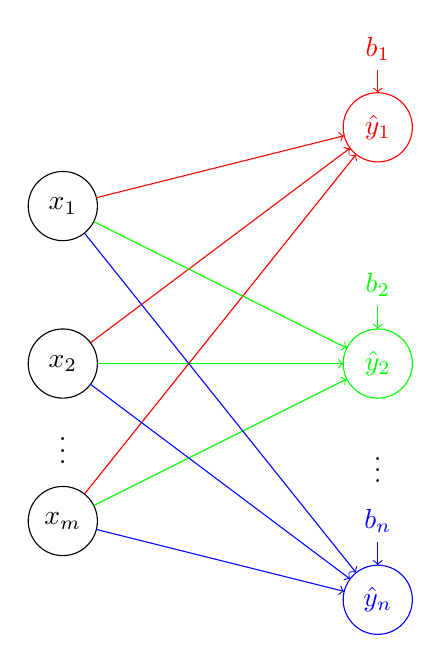
\begin{tikzpicture}
                [
                    neuron/.style = {draw, circle, minimum size=25pt, inner sep=0pt, outer sep=0pt},
                ]
                
                \node [neuron] (x1)  at (0,0) {$x_1$};
                \node [neuron] (x2) at (0,-2) {$x_2$};
                \node (dots) at (0,-3) {$\vdots$};
                \node [neuron] (xm) at (0,-4) {$x_m$};
                \node [neuron,red] (y1) at (4,1) {$\hat{y}_1$};
                \node [neuron,green] (y2) at (4,-2) {$\hat{y}_2$};
                \node [neuron,blue] (yn) at (4,-5) {$\hat{y}_n$};
                \node [red] (b1) at (4, 2) {$b_1$};
                \node [green] (b2) at (4, -1) {$b_2$};
                \node [blue] (bn) at (4, -4) {$b_n$};
                \node (dots) at (4,-3.25) {$\vdots$};
                \draw[->,red] (x1) -- (y1);
                \draw[->,red] (x2) -- (y1);
                \draw[->,red] (xm) -- (y1);
                \draw[->,red] (b1) -- (y1);
                \draw[->,green] (x1) -- (y2);
                \draw[->,green] (x2) -- (y2);
                \draw[->,green] (xm) -- (y2);
                \draw[->,green] (b2) -- (y2);
                \draw[->,blue] (x1) -- (yn);
                \draw[->,blue] (x2) -- (yn);
                \draw[->,blue] (xm) -- (yn);
                \draw[->,blue] (bn) -- (yn);
            \end{tikzpicture}
        \end{center}
        \caption{The DAGs representing the constructions of $n$ SLNs with one output from a SLN with $m$ inputs and $n$ outputs. Each color represents one of the constructed smaller SLNs.}
        \label{fig:sln_m_in_n_out_construction}
    \end{figure}
    
    Now, we can simulate the function of $S$ by the construction
    \begin{equation*}
        S(\vec{x})
        = \begin{bmatrix}
            \hat{y}_1 \\
            \hat{y}_2 \\
            \vdots \\
            \hat{y}_n \\
        \end{bmatrix}
        = \begin{bmatrix}
            S_1(\vec{x}) \\
            S_2(\vec{x}) \\
            \vdots \\
            S_n(\vec{x}) \\
        \end{bmatrix}.
    \end{equation*}
    By Theorem \ref{thm:sln_one_output}, each $S_i$ does not have a linear mapping from weight space to output space, so $S$ cannot have a linear mapping either.
\end{proof}

\begin{corollary}[Weight-output mapping in general]
    \label{col:weight_output_mlp}
    For any MLP $M$, $h_M: \mathcal{W}_M \rightarrow \mathcal{O}_M$ is not a linear mapping.
\end{corollary}
\begin{proof}
    Let $M$ have $L$ layers.
    By Definition \ref{def:mlp}, $M$ is a nested function of $L$ SLNs. 
    Corollary \ref{col:weight_output_sln} states that each of these SLNs does not have a linear mapping from weight to output space.
    Hence the composition of $L$ SLNs that forms $M$ does not have a linear mapping from weight to output space.
\end{proof}

\begin{remark}
    The findings from Corollary \ref{col:weight_output_mlp} are very significant.
    They show that there is no apparent relationship between weight and output space that we can easily determine analytically. 
    If there were a straightforward mapping between weight and output space, we would be able to simply determine the ideal weight configuration that would achieve our target $\vec{y}$ in output space. 
    
    However, since this is not possible, the findings above set the scene for the neural surfing technique. 
    One of the core assumptions is that at a small enough scale, the mapping between weight and output space is \textit{locally linear}, or at least close enough.
\end{remark}

\subsection{Gradient descent from the perspective of weight and output space}
\todo: Write about how SGD with MSE usually gets viewed from the perspective of error-weight surface. However, it is interesting to look at the perspective of weight and output space. It becomes apparent that MSE can be thought of as greedily trying to reduce the Euclidean distance from $\vec{\hat{y}}$ to $\vec{y}$ in output space.

\section{Unrealizable regions}
\begin{definition}[Strongly unrealizable point]
    \label{def:unrealizable_point}
    Given an artificial neural network $A$, a point $\vec{p} \in \mathcal{O}_A$ in output space is \textit{strongly unrealizable} if and only if there exists no weight configuration $\vec{w} \in \mathcal{W}_A$ such that $h_A(\vec{w}) = \vec{p}$.
    In order words, it is impossible to attain $\vec{p}$.
\end{definition}
\begin{definition}[Strongly unrealizable region]
    \label{def:unrealizable_region}
    Given an artificial neural network $A$, a \textit{strongly} unrealizable region $\mathcal{U} \subset \mathcal{O}_A$ is a subspace of the output space where every point $\vec{p} \in \mathcal{U}$ is strongly unrealizable.
    
    It is apparent that there exists no neural learning algorithm that can elicit a change in weight space that will attain a point in a strongly unrealizable region in output space.
    Hence we define a \textit{weakly} unrealizable region for a particular neural learning algorithm as a region in output space that cannot be attained by a particular algorithm.
\end{definition}

\begin{lemma}
    A strongly unrealizable region cannot encompass the whole output space.
\end{lemma}
\begin{proof}
    Let us consider an artifical neural network $A$. 
    We will show that for every unrealizable region, $\mathcal{U} \subsetneq \mathcal{O}_A$.
    By Definition \ref{def:unrealizable_region}, $\mathcal{U} \subset \mathcal{O}_A$, so it remains to prove that every unrealizable region $\mathcal{U} \neq \mathcal{O}_A$.

    Choose any weight configuration $\vec{w} \in \mathcal{W}_A$. 
    Let the point $\vec{p}=h_A(\vec{w})$. 
    We know that $\vec{p}$ is \textit{not} strongly unrealizable because $\vec{w}$ achieves $\vec{p}$. 
    Hence no unrealizable region can contain $\vec{p}$, so $\vec{p} \notin \mathcal{U}$ but $\vec{p} \in \mathcal{O}_A$. 
    It follows that $\mathcal{U} \neq \mathcal{O}_A$.
\end{proof}

Let us look at a couple of examples of unrealizable regions.
\begin{example}
    A trivial example of an unrealizable region is predicting two different outputs for the same training sample.
    Consider again an MLP $M$ with one layer and two inputs, as shown in Figure \ref{fig:sln_2_in_1_out}.
    Let $\vec{x}\in \mathbb{R}^2$ be any point in input space.
    For this example, let the training data be the matrix
    $
        \vec{X} = \begin{bmatrix}
            \vec{x} & \vec{x}
        \end{bmatrix}\tran
    $.
    Now we can define an unrealizable region
    \begin{equation*}
        \mathcal{U} = \left\{
            \begin{bmatrix}
                p_1 \\ p_2
            \end{bmatrix} : p_1, p_2 \in \mathbb{R}, p_1 \neq p_2
        \right\}
    \end{equation*}
    because $h_M(\vec{x})$ cannot produce two different outputs for the same value of $\vec{x}$.
\end{example}
\begin{example}[XOR mapping]
    Let us look at a less contrived example.
    While it ``is well known that any Boolean function \elide can be approximated by a suitable two-layer feed-forward network'' \cite{blum1989}, 
    single-layer networks with non-decreasing activation functions can only learn a Boolean mapping that is \textit{linearly separable} \cite[p. 723]{russell2010}.
    A linearly separable mapping has a linear decision boundary which means that there is only one linear hyperplane separating the two classes (true and false).
    
    The XOR function is not linearly separable because it requires at least two linear decision boundaries, as shown in Figure \ref{fig:xor}.
    \begin{figure}
        \centering
        \begin{tikzpicture}
            \begin{axis}[
                x=2cm,
                y=2cm,
                axis lines=center,
                xlabel={$x_1$}, xlabel style={anchor=west},
                ylabel={$x_2$}, ylabel style={anchor=south},
                ymin=0, ymax=1.7,
                xmin=0, xmax=1.7,
                samples=100,
                xtick={0, 1},
                ytick={0, 1},
                extra x ticks=0,
                extra x tick style={
                    tick label style={
                        anchor=north east,
                        xshift=-.5*\pgfkeysvalueof{/pgfplots/major tick length}
                }}
            ]
                \addplot[black,only marks,mark=*] coordinates {(0,1) (1,0)};
                \addplot[black,only marks,mark=o] coordinates {(0,0) (1,1)};
                \addplot[black, no marks] coordinates {(0,.5) (.5,0)};
                \addplot[black, no marks] coordinates {(0,1.5) (1.5,0)};
                \addplot[black, ->] coordinates {(.25,.25) (.35,.35)};
                \addplot[black, ->] coordinates {(.75,.75) (.65,.65)};
            \end{axis}
        \end{tikzpicture}
        \caption{The locations of the two hyperplanes in input space acting as decision boundaries required to learn an XOR mapping. The filled-in dot represents an activation of 1 (true) and the circle represents 0 activation (false).}
        \label{fig:xor}
    \end{figure}
    We will consider the same single-layer architecture from Figure \ref{fig:sln_2_in_1_out} again, using the sigmoid activation function.
    The sigmoid is a non-decreasing function.
    Since we only have one unit (the output neuron) with this non-decreasing non-linear activation function, it follows that we can only have one decision boundary.
    We just showed that the XOR mapping requires two decision boundaries.
    Therefore, given the input matrix
    \begin{equation*}
        \vec{X} = \begin{bmatrix}
            0 & 0 \\
            0 & 1 \\
            1 & 0 \\
            1 & 1
        \end{bmatrix},
    \end{equation*}
    the point
    $
        \vec{p} = \begin{bmatrix}
            0 & 1 & 1 & 0
        \end{bmatrix}\tran
    $
    in output space is strongly unrealizable.
    So $\mathcal{U} = \{\vec{p}\}$ is an example of an unrealizable region.    
\end{example}





\todo: Explain significance if target is unrealizable (XOR example demonstrates that)

\section{Goal-connecting paths}
\begin{definition}[Goal-connecting path]
    For an artificial neural network $A$ with current weight configuration $\vec{w}_0 \in \mathcal{W}_A$, a goal-connecting path in output space to the goal $\vec{g}\in \mathcal{O}_A$ is a sequence of points $\vec{s}_0, \vec{s}_1,\dots,\vec{s}_{S} \in \mathcal{O}_A$ where the initial state $\vec{s}_0 = h_A(\vec{w}_0)$ and final state $\vec{s}_S=\vec{g}$.
    The points $\vec{s}_1,\vec{s}_2,\dots,\vec{s}_S$ are referred to as \textit{subgoals}, hence $S$ is the number of subgoals in the goal-connecting path. 

    The goal-connecting path is \textit{realizable} if and only if no subgoal is a strongly unrealizable point (Definition \ref{def:unrealizable_point}).
    This means that a realizable goal-connecting path can equivalently be defined by the weight configurations $\vec{w}_0, \vec{w_1},\dots,\vec{w}_S \in \mathcal{W}_A$ such that $h_A(\vec{w}_i) = \vec{s}_i$ for $i \leq S$.
\end{definition}

\begin{definition}[Ideal goal-connecting path]
    \label{def:ideal_goal_connecting_path}
    The ideal goal-connecting path of $S$ subgoals for an artifical neural network $A$ is, in terms of weight space, the \textit{shortest} realizable goal-connecting path with equidistant subgoals. 
\end{definition}

\begin{lemma}
    \label{lmm:ideal_subgoal_construction}
    Given $\vec{w}_0$ and $\vec{w}_S$, the $i$th subgoal of the ideal goal-connecting path in weight space is given by
    $
        \vec{w}_i = \vec{w}_0 + \frac{i}{S}\left( \vec{w}_S - \vec{w}_0 \right)
    $.
\end{lemma}
\begin{proof}
    First, we will show that the points are equidistant, i.e. $\norm{\vec{w}_0 - \vec{w}_1} = \norm{\vec{w}_1 - \vec{w}_2} = \dots = \norm{\vec{w}_{S-1} - \vec{w}_S}$.
    This is equivalent to asserting that $\norm{\vec{w}_{i-1} - \vec{w}_i} = \norm{\vec{w}_i - \vec{w}_{i+1}}$ for $0 < i < S$.
    Substituting on the LHS,
    \begin{align*}
        \norm{\vec{w}_{i-1} - \vec{w}_i}
        &= \norm{\vec{w}_0 + \frac{i-1}{S}\left( \vec{w}_S - \vec{w}_0 \right) - \vec{w}_0 - \frac{i}{S}\left( \vec{w}_S - \vec{w}_0 \right)} \\
        &= \norm{-\frac{1}{S}\left(\vec{w}_S - \vec{w}_0 \right)},
    \end{align*}
    and on the RHS,
    \begin{align*}
        \norm{\vec{w}_i - \vec{w}_{i+1}}
        &= \norm{\vec{w}_0 + \frac{i}{S}\left( \vec{w}_S - \vec{w}_0 \right) - \vec{w}_0 - \frac{i+1}{S}\left( \vec{w}_S - \vec{w}_0 \right)} \\
        &= \norm{-\frac{1}{S}\left(\vec{w}_S - \vec{w}_0 \right)}.
    \end{align*}

    The shortest path between two points is a straight line, so the ideal goal-connecting path in weight space must form a straight line from $\vec{w}_0$ to $\vec{w}_S$, and all subgoals must lie on this line.
    The equation of the line $l:\mathbb{R} \rightarrow \mathcal{W}_A$ from $\vec{w}_0$ to $\vec{w}_S$ is $l(\lambda) = \vec{w}_0 + \lambda\left( \vec{w}_S - \vec{w}_0 \right)$.
    It is easy to see that $l\left(\frac{i}{S}\right)=\vec{w}_i$ for $0 \leq i \leq S$, so the subgoals are collinear.
\end{proof}

\begin{remark}
    Lemma \ref{lmm:ideal_subgoal_construction} shows a construction for achieving the ideal goal-connecting path, given knowledge of the target weight configuration $\vec{w}_S$.
    Of course, this is not known to the neural learning algorithm while it is learning, only once it finished and was able to actually achieve the goal. 
    However, we can use the ideal goal-connecting path in retrospect to evaluate the performance of the neural learning algorithm in comparison to the ideal path.
    Furthermore, we can plot the ideal goal-connecting path in output space in order to find unrealizable regions.
\end{remark}

\chapter{Problems}

\section{The stripe problem}
\label{sec:stripe_problem}
The stripe problem provides a practical example of the local minimum problem. 
We will consider a two-dimensional input space with two (initially) parallel hyperplanes that form a stripe.
The initial configuration will have the hyperplanes arranged horizontally and misclassify some of the samples. 
Changing the weights in the neural network will allow the hyperplanes to rotate, but when they do so, they are forced to misclassify even more samples (thereby increasing the mean squared error) until eventually reaching the target configuration with zero error.

The stripe problem can be achieved by a 2-2-1 sigmoidal MLP \cite{weir2019}. 
Figure \ref{fig:stripe_original_hyperplanes} shows the initial and target configurations of the hyperplanes for this type of network.
The hidden layer is required because without it, the sigmoid activation function will produce only one hyperplane, as proved in Lemma \ref{lmm:sigmoid_decision_boundary}.
\begin{figure}
    \centering
    \begin{subfigure}{.45\textwidth}
        \begin{tikzpicture}
            \begin{axis}[
                x=1cm,
                y=1cm,
                axis lines=center,
                xlabel={$x_1$}, xlabel style={anchor=west},
                ylabel={$x_2$}, ylabel style={anchor=south},
                ymin=0, ymax=4.2,
                xmin=0, xmax=4.2,
                grid=none,
                samples=100,
                ticks=none
            ]
                \addplot[black,only marks,mark=*] coordinates {(2,1.5) (2,2.5)};
                \addplot[black,only marks,mark=o] coordinates {(2,.5) (.5,.5) (3.5,.5) (.5,3.5) (3.5,3.5) (2,3.5)};
                \addplot[black, no marks] coordinates {(0,1) (4,1)};
                \addplot[black, no marks] coordinates {(0,3) (4,3)};
                \addplot[black, ->] coordinates {(1,1) (1,1.35)};
                \addplot[black, ->] coordinates {(1,3) (1,2.65)};
            \end{axis}
        \end{tikzpicture}
        \caption{Initial configuration}
    \end{subfigure}
    \hspace*{\fill}
    \begin{subfigure}{.45\textwidth}
        \begin{tikzpicture}
            \begin{axis}[
                x=1cm,
                y=1cm,
                axis lines=center,
                xlabel={$x_1$}, xlabel style={anchor=west},
                ylabel={$x_2$}, ylabel style={anchor=south},
                ymin=0, ymax=4.2,
                xmin=0, xmax=4.2,
                grid=none,
                samples=100,
                ticks=none
            ]
                \addplot[black,only marks,mark=*] coordinates {(2,.5) (2,1.5) (2,2.5) (2,3.5)};
                \addplot[black,only marks,mark=o] coordinates {(.5,.5) (3.5,.5) (.5,3.5) (3.5,3.5)};
                \addplot[black, no marks] coordinates {(1,0) (1,4)};
                \addplot[black, no marks] coordinates {(3,0) (3,4)};
                \addplot[black, ->] coordinates {(1,1) (1.35,1)};
                \addplot[black, ->] coordinates {(3,1) (2.65,1)};
            \end{axis}
        \end{tikzpicture}
        \caption{Target configuration}
    \end{subfigure}
    \caption{Hyperplanes in input space for the stripe problem with eight samples (adapted from \textcite{weir2019}).}
    \label{fig:stripe_original_hyperplanes}
\end{figure}

In this section, we will formulate a version of the stripe problem that requires no hidden layers and fewer input samples by using a different kind of activation function.
The reduced number of parameters will lend itself better for analysis.

\subsection{Radial basis activation functions}
We will first introduce the concept of radial basis functions. 
When used as the activation function, they exhibit some advantageous properties that will aid us to contrive a simple version of the stripe problem.
\begin{definition}[Radial basis function]
    \label{def:rbf}
    A radial basis function (RBF) is a smooth continuous real-valued\footnote{We define RBFs has having a scalar domain and range because this suffices for our purposes. In actual fact, RBFs are defined more generally to map between suitable vector spaces \cite{buhmann2000}.} function $\phi : \mathbb{R} \rightarrow \mathbb{R}$ that satisfies the property $\phi(x) = \phi(\norm{x})$ \cite{buhmann2000}. 
    %RBFs are commonly used as a kernel in support vector machines (SVMs) \cite{burkov2019}.
    For RBFs to be useful activation functions, we three additional restrictions:
    \begin{enumerate*}[label=(\roman*)]
        \item $\phi(0)=1$;
        \item $\phi(x)$ is strictly increasing for $x<0$ when $\phi(x) \neq 0$; and
        \item that
    \end{enumerate*}
    \begin{equation*}
        \lim_{x\rightarrow -\infty}{\phi(x)} = \lim_{x\rightarrow \infty}{\phi(x)} = 0.
    \end{equation*}
\end{definition}

Two commonly used RBFs, both infinitely differentiable, are the Gaussian function
\begin{equation}
    \label{eq:gaussian}
    \phi(x) = e^{-x^2}
\end{equation}
and the bump function\footnote{We give a slightly modified version of the well-known $C_\infty$ ``bump'' function \cite{johnson2015} that is vertically scaled such that $\phi(0)=1$ for convenience.}
\begin{equation}
    \label{eq:bump}
    \phi(x) = 
    \begin{cases}
        e^{1-\frac{1}{1-x^2}} & \text{for $-1<x<1$} \\
        0 & \text{otherwise}
    \end{cases}.
\end{equation}
These functions, graphed in Figure \ref{fig:rbfs}, exhibit slightly different properties.
\begin{figure}
    \centering
    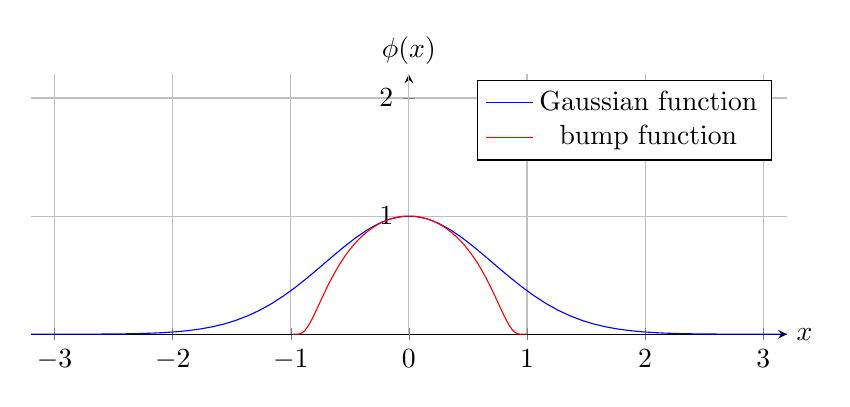
\begin{tikzpicture}[
        declare function={
            gaussian(\x)= exp(-\x^2);
            bump(\x)= and(\x>=-1, \x<=1) * exp(1-1/(1-(\x^2)));
        }
    ]
        \begin{axis}[
            x=1.5cm,
            y=1.5cm,
            axis lines=center,
            xlabel={$x$}, xlabel style={anchor=west},
            ylabel={$\phi(x)$}, ylabel style={anchor=south},
            ymin=0, ymax=2.2,
            xmin=-3.2, xmax=3.2,
            grid,
            samples=100,
            xtick={-3,...,3},
            ytick={0, 1, 2},
            extra x ticks = 0
        ]
            \addplot[blue] {gaussian(x)};
            \addplot[red,domain=-1:1] {bump(x)};
            \legend{Gaussian function,bump function}
        \end{axis}
    \end{tikzpicture}
    \caption{Plots of the two most common radial basis functions.}
    \label{fig:rbfs}
\end{figure}
The Gaussian function never actually reaches zero and its derivative is never zero (except at the peak, i.e. $x=0$). 
On the other hand, for the bump function, we have $\phi(x)=0$ and $\frac{d\phi}{dx}=0$ for $x \notin (-1, 1)$.

\begin{lemma}[Single-layer RBF decision boundaries]
    \label{lmm:single_layer_rbf_decision_boundaries}
    A single-layer Gaussian RBF MLP with decision threshold $t\in (0,1)$ will have two hyperplanes in input space.
\end{lemma}
\begin{proof}
    The proof is similar in method as in Lemma \ref{lmm:sigmoid_decision_boundary}.
    Consider an equivalent SLN $S$ with $m$ inputs and one output as shown in Figure \ref{fig:sln_m_in_1_out}. 
    To obtain the decision boundaries, we set the output equal to the decision threshold, so
    \begin{align*}
        t &= S\left(\vec{x}\right) \\
        &= \phi\left(\vec{w}\tran \vec{x} + b\right) \\
        &= e^{-\left(\vec{w}\tran \vec{x} + b \right)^2} \\
        -\ln{t} &= \left(\vec{w}\tran \vec{x} + b \right)^2 \\
        \pm \sqrt{-\ln{t}} &= \vec{w}\tran \vec{x} + b.
    \end{align*}
    Since $t\in (0,1)$, it follows that
    \begin{align*}
        0 < t &< 1 \\
        \ln t &< \ln 1 \\
        -\ln t &> 0 \\
        \sqrt{-\ln{t}} &> 0
    \end{align*}
    which means that $\sqrt{-\ln{t}} \neq 0$. 
    Hence
    \begin{equation}
        \label{eq:gaussian_hyperplanes}
        \vec{w}\tran \vec{x} + b \pm \sqrt{-\ln{t}} = 0
    \end{equation}
    has two distinct solutions, no matter the values of $\vec{w}$, $\vec{x}$, and $b$.
    Thus there will always be two hyperplanes.
\end{proof}
\begin{remark}
    Although Lemma \ref{lmm:single_layer_rbf_decision_boundaries} proves the existence of two hyperplane decision boundaries for Gaussian RBFs, it is trivial to modify this proof for any other type of RBF, such as the bump function.
    As a consequence, we know that unlike single-layer sigmoidal networks (see Lemma \ref{lmm:sigmoid_decision_boundary}), we can use single-layer RBF networks to generate a decision boundary in the form of a stripe which will allow us to use this type of network to provide a more simple example of the stripe problem.
\end{remark}

\begin{example}
    \label{ex:sln_2_in_1_out_gaussian_hyperplanes}
    Like in Example \ref{ex:sln_2_in_1_out_sigmoid_hyperplane}, let us consider once more a single-layered MLP $M$ with two inputs, depicted in Figure \ref{fig:sln_2_in_1_out}, where $w_1=w_2=1$ and $b=0$. 
    Let the threshold be $t=\frac{1}{2}$ again, but this time, we will use the Gaussian RBF as the activation function.

    From (\ref{eq:gaussian_hyperplanes}), we obtain the equations of the hyperplanes as
    \begin{align*}
        \vec{w}\tran \vec{x} + b \pm \sqrt{-\ln{\frac{1}{2}}} &= 0 \\
        w_1 x_1 + w_2 x_2 + b &=  \pm \sqrt{-\ln{\frac{1}{2}}} \\
        x_1 + x_2 &= \pm \sqrt{-\ln{\frac{1}{2}}},
    \end{align*}
    so the hyperplanes are at $x_2 = -x_1 - 0.8325\dots$ and $x_2 = -x_1 + 0.8325\dots$, as shown in Figure \ref{fig:gaussian_hyperplanes}.

    \begin{figure}
        \begin{subfigure}[b]{0.45\textwidth}
            \begin{tikzpicture}[
                declare function={
                    hminus(\x)= -\x - sqrt(-ln(0.5));
                    hplus(\x)= -\x + sqrt(-ln(0.5));
                }
            ]
                \begin{axis}[
                    scale only axis,
                    width=.8\textwidth,
                    axis lines=center,
                    xlabel={$x_1$}, xlabel style={anchor=west},
                    ylabel={$x_2$}, ylabel style={anchor=south},
                    ymin=-2.5, ymax=2.5,
                    xmin=-2.5, xmax=2.5,
                    samples=2
                ]
                    \addplot[black,only marks,mark=*] coordinates {(0,0) (-1,1) (1,-1)};
                    \addplot[black,only marks,mark=o] coordinates {(1,1) (-1, 2.2) (1.5,0) (0,1.5) (2.2,1) (1,2.2) (2.2,-1) (-1,-1) (1, -2.2) (-1.5,0) (0,-1.5) (-2.2,-1) (-1,-2.2) (-2.2,1)};
                    \addplot[black, no marks] {hminus(x)};
                    \addplot[black, no marks] {hplus(x)};
                    \addplot[black, ->] coordinates {(-2,{hminus(-2)}) (-1.75, {2*hminus(-2)-hminus(-1.75)})};
                    \addplot[black, ->] coordinates {({-hminus(-2)},{hplus(-hminus(-2))}) ({-hminus(-2)-.25}, {2*hplus(-hminus(-2))-hplus(-hminus(-2)-.25)})};
                \end{axis}
            \end{tikzpicture}
            \vspace{.5cm}
            \caption{Input space with sample data}
        \end{subfigure}
        \hspace*{\fill}
        \begin{subfigure}[b]{0.55\textwidth}
            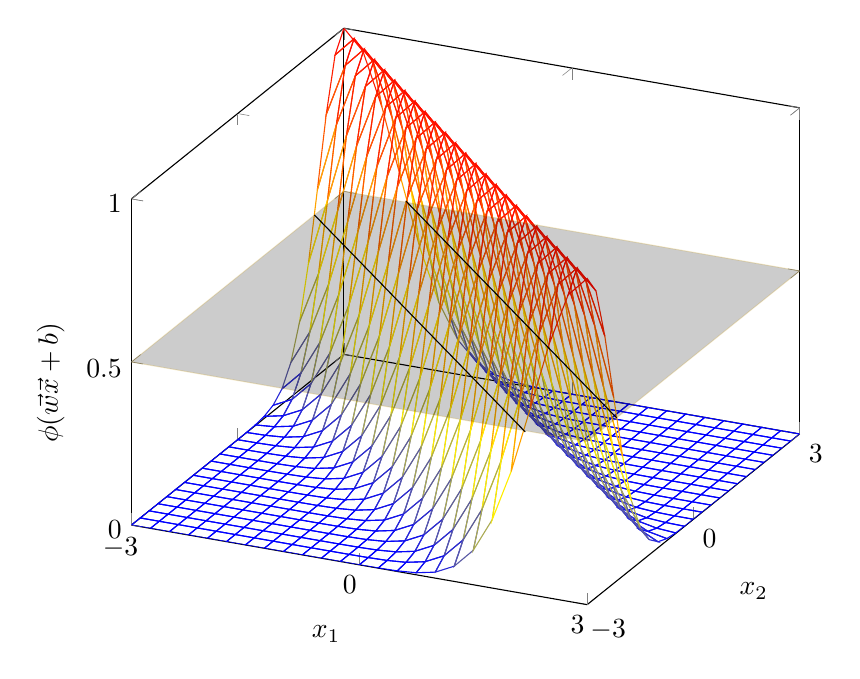
\begin{tikzpicture}
                \begin{axis}[
                    scale only axis,
                    width=.7\textwidth,
                    ymin=-3, ymax=3,
                    xmin=-3, xmax=3,
                    zmin=0, zmax=1,
                    xlabel={$x_1$},
                    ylabel={$x_2$},
                    zlabel={$\phi(\vec{w}\tran \vec{x} + b)$},
                    samples=25,
                    xtick={-3,0,3},
                    ytick={-3,0,3},
                    ztick={0, 1},
                    extra z ticks={0.5}
                ]
                    \addplot3 [
                        mesh,
                        domain=-3:3,
                        y domain=-3:3,
                    ] {exp(-(x+y)^2)};
                    \addplot3 [
                        surf,
                        fill=black,
                        opacity=0.2,
                        domain=-3:3,
                        y domain=-3:3,
                        samples=2
                    ] {.5};
                    \addplot3[
                        samples=2,
                        mark=none,
                        domain=-3:2.2,
                        y domain=-3:3
                    ] ({x}, {-x - sqrt(-ln(0.5))}, {0.5});
                    \addplot3[
                        samples=2,
                        mark=none,
                        domain=-2.2:3,
                        y domain=-3:3
                    ] ({x}, {-x + sqrt(-ln(0.5))}, {0.5});
                \end{axis}
            \end{tikzpicture}
            \caption{Input-activation space}
        \end{subfigure}
        \caption{Plots of the hyperplanes of the MLP from Figure \ref{fig:sln_2_in_1_out} with Gaussian RBF activation where $w_1=w_2=1$, $b=0$.}
        \label{fig:gaussian_hyperplanes}
    \end{figure}
\end{example}
\begin{remark}
    One key realisation is that when $w_1$ is fixed, changing the value of $w_2$ will result in both hyperplanes being rotated around their respective $x_1$-intercepts (the hyperplanes remain parallel).
    The same is true vice-versa, except that the hyperplanes are rotated around their $x_2$-intercepts.
    Changing the value of $b$ simply translates the hyperplanes linearly in input space.
\end{remark}

\subsection{Formulating the problem}
Example \ref{ex:sln_2_in_1_out_gaussian_hyperplanes} showed that a simple 2-1 network with radial basis activation constructs a scenario where the hyperplanes form a stripe that can be rotated by adjusting the weights.
This means that we could easily contrive the stripe problem from Figure \ref{fig:stripe_original_hyperplanes}.
However, since we established that the hyperplanes will always remain parallel in our RBF network and since they rotate around the origin when $b$ is fixed, we can create a much simplified version of the stripe problem using only four samples.

\begin{figure}
    \centering
    \begin{subfigure}{.45\textwidth}
        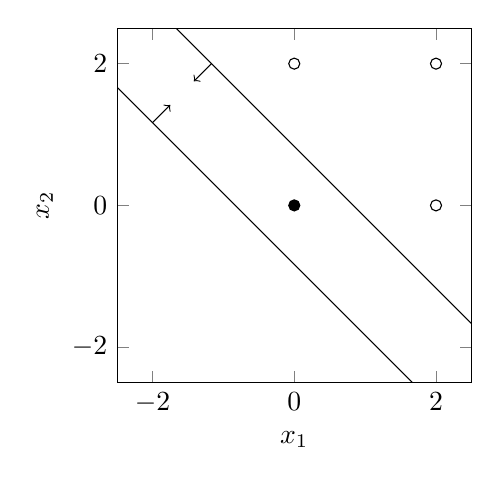
\begin{tikzpicture}[
            declare function={
                hminus(\x)= -\x - sqrt(-ln(0.5));
                hplus(\x)= -\x + sqrt(-ln(0.5));
            }
        ]
            \begin{axis}[
                x=.9cm,
                y=.9cm,
                xlabel={$x_1$},
                ylabel={$x_2$},
                ymin=-2.5, ymax=2.5,
                xmin=-2.5, xmax=2.5,
                samples=2
            ]
                \addplot[black,only marks,mark=*] coordinates {(0,0)};
                \addplot[black,only marks,mark=o] coordinates {(0,2) (2,0) (2,2)};
                \addplot[black, no marks] {hminus(x)};
                \addplot[black, no marks] {hplus(x)};
                \addplot[black, ->] coordinates {(-2,{hminus(-2)}) (-1.75, {2*hminus(-2)-hminus(-1.75)})};
                \addplot[black, ->] coordinates {({-hminus(-2)},{hplus(-hminus(-2))}) ({-hminus(-2)-.25}, {2*hplus(-hminus(-2))-hplus(-hminus(-2)-.25)})};
            \end{axis}
        \end{tikzpicture}
        \caption{Initial configuration}
    \end{subfigure}
    \hspace*{\fill}
    \begin{subfigure}{.45\textwidth}
        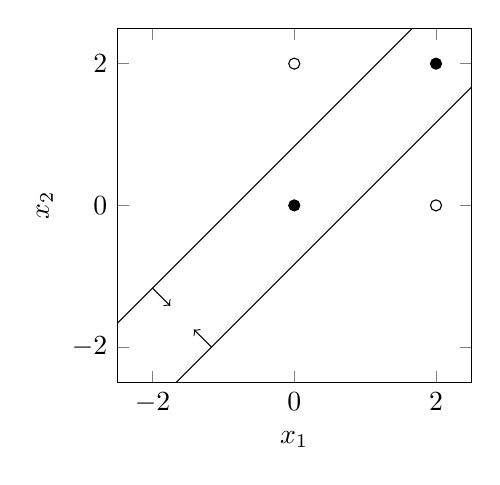
\begin{tikzpicture}[
            declare function={
                hminus(\x)= \x + sqrt(-ln(0.5));
                hplus(\x)= \x - sqrt(-ln(0.5));
            }
        ]
            \begin{axis}[
                x=.9cm,
                y=.9cm,
                xlabel={$x_1$},
                ylabel={$x_2$},
                ymin=-2.5, ymax=2.5,
                xmin=-2.5, xmax=2.5,
                samples=2
            ]
                \addplot[black,only marks,mark=*] coordinates {(0,0) (2,2)};
                \addplot[black,only marks,mark=o] coordinates {(0,2) (2,0)};
                \addplot[black, no marks] {hminus(x)};
                \addplot[black, no marks] {hplus(x)};
                \addplot[black, ->] coordinates {(-2,{hminus(-2)}) (-1.75, {2*hminus(-2)-hminus(-1.75)})};
                \addplot[black, ->] coordinates {({hminus(-2)},{hplus(hminus(-2))}) ({hminus(-2)-.25}, {2*hplus(hminus(-2))-hplus(hminus(-2)-.25)})};
            \end{axis}
        \end{tikzpicture}
        \caption{Target configuration}
    \end{subfigure}
    \caption{The hyperplanes in the initial and target configurations of the RBF stripe problem.}
    \label{fig:stripe_hyperplanes}
\end{figure}
Figure \ref{fig:stripe_hyperplanes} depicts the initial and target configurations of this simplified version. 
It is obvious that whichever direction the stripe rotates, it will need to misclassify one of the samples before achieving the target configuration.

\begin{table}[h!]
    \centering
    \begin{tabular}{c|c|c}
        input ($\vec{x}$) & target output ($y$) & initial output ($\hat{y}$) \\
        \hline
        $\begin{bmatrix} 0 & 0 \end{bmatrix}$
        & 1 & 1
        \\
        $\begin{bmatrix} 2 & 2 \end{bmatrix}$
        & 1 & $\phi\left( 4 \right)$
        \\
        $\begin{bmatrix} 0 & 2 \end{bmatrix}$
        & $\phi\left( 2 \right)$ & $\phi\left( 2 \right)$
        \\
        $\begin{bmatrix} 2 & 0 \end{bmatrix}$
        & $\phi\left(2 \right)$ & $\phi\left( 2 \right)$
    \end{tabular}
    \caption{The dataset for the RBF stripe problem.}
    \label{table:stripe_dataset}
\end{table}
We give the dataset for the stripe problem in Table \ref{table:stripe_dataset}.
Notice that the third and fourth samples do not have a target output of zero, but rather $\phi(2)$ which is close to zero (for the Gaussian RBF, $\phi(2) \approx 0.018$, and for the bump function $\phi(2) = 0$).
This will make some calculations later more convenient because it guarantees that there exists at least one weight configuration with a MSE of zero.

\begin{figure}
    \centering
    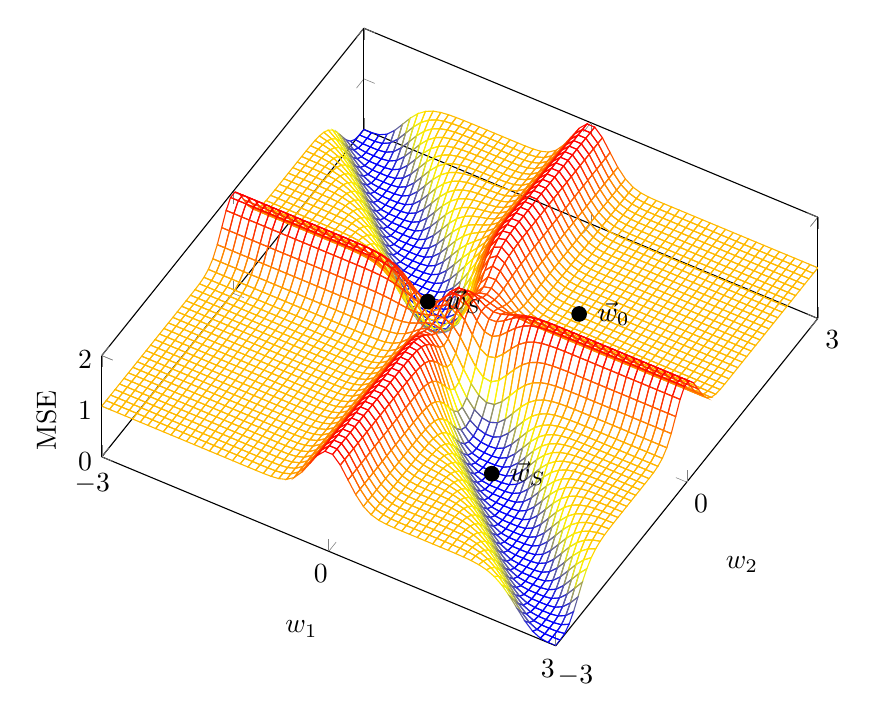
\begin{tikzpicture}[
        declare function={
            rbf(\x)= exp(-\x^2);
        }
    ]
        \begin{axis}[
            scale only axis,
            width=.75\textwidth,
            ymin=-3, ymax=3,
            xmin=-3, xmax=3,
            zmin=0, zmax=2,
            xlabel={$w_1$},
            ylabel={$w_2$},
            zlabel={MSE},
            samples=60,
            xtick={-3,0,3},
            ytick={-3,0,3},
            ztick={0, 1, 2},
            view={30}{75}
        ]
            \addplot3 [
                mesh,
                domain=-3:3,
                y domain=-3:3
            ] {(rbf(2*x) - rbf(2))^2 + (rbf(2*y) - rbf(2))^2 + (rbf(2*x + 2*y) - 1)^2};
            \node[label={360:{$\vec{w}_0$}},circle,fill,inner sep=2pt] at (1, 1, 1) {};
            \node[label={360:{$\vec{w}_S$}},circle,fill,inner sep=2pt] at (1, -1, 0) {};
            \node[label={360:{$\vec{w}_S$}},circle,fill,inner sep=2pt] at (-1, 1, 0) {};
        \end{axis}
    \end{tikzpicture}
    \caption{Error-weight surface of the stripe problem with Gaussian activation.}
    \label{fig:stripe_error_surface_gaussian}
    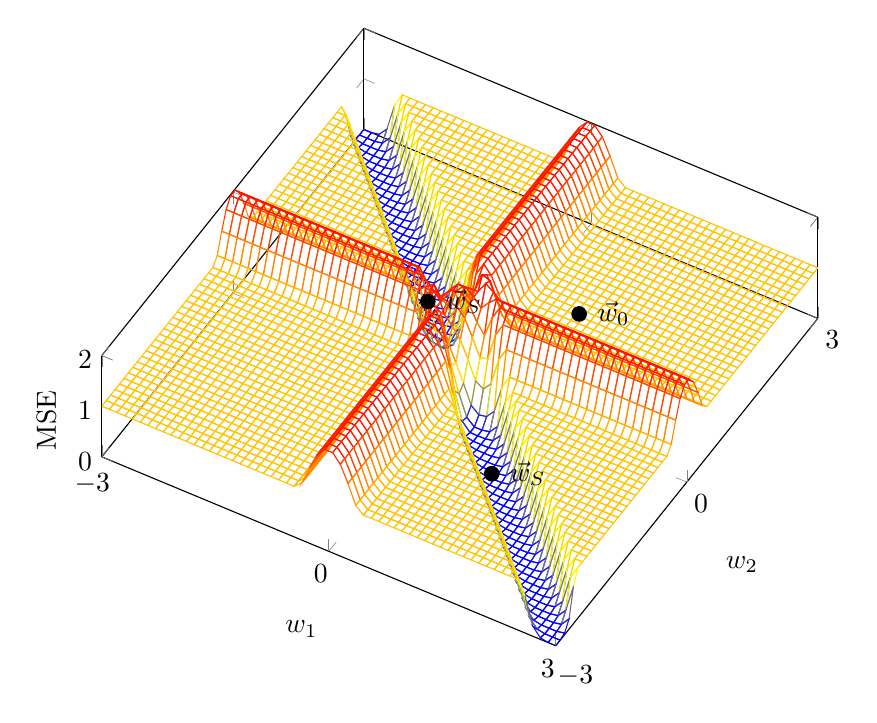
\begin{tikzpicture}[
        declare function={
            rbf(\x)= and(\x>=-1, \x<=1) * exp(1-1/(1-(\x^2)));
        }
    ]
        \begin{axis}[
            scale only axis,
            width=.75\textwidth,
            ymin=-3, ymax=3,
            xmin=-3, xmax=3,
            zmin=0, zmax=2,
            xlabel={$w_1$},
            ylabel={$w_2$},
            zlabel={MSE},
            samples=60,
            xtick={-3,0,3},
            ytick={-3,0,3},
            ztick={0, 1, 2},
            view={30}{75}
        ]
            \addplot3 [
                mesh,
                domain=-3:3,
                y domain=-3:3
            ] {(rbf(2*x) - rbf(2))^2 + (rbf(2*y) - rbf(2))^2 + (rbf(2*x + 2*y) - 1)^2};
            \node[label={360:{$\vec{w}_0$}},circle,fill,inner sep=2pt] at (1, 1, 1) {};
            \node[label={360:{$\vec{w}_S$}},circle,fill,inner sep=2pt] at (1, -1, 0) {};
            \node[label={360:{$\vec{w}_S$}},circle,fill,inner sep=2pt] at (-1, 1, 0) {};
        \end{axis}
    \end{tikzpicture}
    \caption{Error-weight surface of the stripe problem with bump activation.}
    \label{fig:stripe_error_surface_bump}
\end{figure}
Let us examine the error-weight surface of the stripe problem. 
It is depicted in Figures \ref{fig:stripe_error_surface_gaussian} and \ref{fig:stripe_error_surface_bump} for the Gaussian and bump activation functions, respectively.
The graphs are quite similar, showing that the initial weight configuration $\vec{w}_0$ has a MSE of around $1$.
Most importantly, we see that in order to get to any of the goal weight states $\vec{w}_S$ in the region where the MSE is close to zero, we must first overcome a `hill'.

For the remainder of this project, we will consider only the Gaussian RBF function, but let it be noted that in principle, any type of RBF that satisfies the criteria given in Definition \ref{def:rbf} is suitable.
The Gaussian RBF, however, lends itself better for the purposes of analysis because it is not a piecewise defined function, and it does not have a derivative of zero anywhere except at $x=0$. 
In addition, gradient descent fails immediately with the bump function because the initial weight configuration is at an area where the gradient is exactly zero.
Henceforth the term `stripe problem' shall be used to refer to the Gaussian RBF version of the stripe problem. 

\subsection{Local minima}
We will now attempt to find the local minima in the error-weight surface analytically. 
From Table \ref{table:stripe_dataset} we obtain the input matrix
\begin{equation*}
    \vec{X} = \begin{bmatrix}
        0 & 0 \\
        2 & 2 \\
        0 & 2 \\
        2 & 0
    \end{bmatrix}
\end{equation*}
and target output vector
$\vec{y} = \begin{bmatrix}
    1 & 1 & \phi(2) & \phi(2)
\end{bmatrix}\tran$.
Modifying the SLN function from Definition \ref{def:sln} for the case of our 2-1 RBF network without bias, we have $S(\vec{x}) = \phi(\vec{w}\tran \vec{x})$.
This means that our loss function is given by
\begin{align*}
    L(\vec{w}) = L
    &= \sum_{i=1}^4{\left(\phi\left(\vec{w}\tran \vec{x}_i\right) - y_i\right)^2} \\
    &= \left(\phi(\vec{w}\tran\vec{x}_1) - 1\right)^2
     + \left(\phi(\vec{w}\tran\vec{x}_2) - 1\right)^2 \\
    &\qquad+ \left(\phi(\vec{w}\tran\vec{x}_3) - \phi(2)\right)^2
     + \left(\phi(\vec{w}\tran\vec{x}_4) - \phi(2)\right)^2 \\
    &= \left(\phi(0) - 1\right)^2
     + \left(\phi(2 w_1 + 2 w_2) - 1\right)^2 \\
    &\qquad+ \left(\phi(2 w_2) - \phi(2)\right)^2
     + \left(\phi(2 w_1) - \phi(2)\right)^2.
\end{align*}
Substituting (\ref{eq:gaussian}), we obtain
\begin{equation}
    L
     = \left(e^{-(2 w_1 + 2 w_2)^2} - 1\right)^2
     + \left(e^{-(2 w_2)^2} - e^{-4}\right)^2
     + \left(e^{-(2 w_1)^2} - e^{-4}\right)^2.
\end{equation}

\begin{lemma}
    The three critical points of the error-weight surface given by $L$ are 
    $\vec{w}_1 = \begin{bmatrix}
        -1 & 1
    \end{bmatrix}\tran$,
    $\vec{w}_2 = \begin{bmatrix}
        1 & -1
    \end{bmatrix}\tran$, and
    $\vec{w}_3 = \begin{bmatrix}
        0 & 0
    \end{bmatrix}\tran$.
\end{lemma}

\begin{proof}
    We need to find the Jacobian, $\vec{J}_L$. 
    Differentiating $L$ with respect to $w_1$ gives
    \begin{align*}
        \frac{\delta L}{\delta w_1}
        &= 2 \left(e^{-(2 w_1 + 2 w_2)^2} - 1\right) \frac{\delta}{\delta w_1} e^{-(2 w_1 + 2 w_2)^2} \\
        &\qquad + 2 \left(e^{-(2 w_1)^2} - e^{-4}\right) \frac{\delta}{\delta w_1} e^{-(2 w_1)^2} \\
        &= -16 \left(e^{-(2 w_1 + 2 w_2)^2} - 1\right) \left(w_1 + w_2 \right) e^{-(2 w_1 + 2 w_2)^2} \\
        &\qquad -16 w_1 \left(e^{-4 w_1^2} - e^{-4}\right) e^{-4 w_1^2},
    \end{align*}
    and for $w_2$ we have
    \begin{align*}
        \frac{\delta L}{\delta w_2}
        &= 2 \left(e^{-(2 w_1 + 2 w_2)^2} - 1\right) \frac{\delta}{\delta w_2} e^{-(2 w_1 + 2 w_2)^2} \\
        &\qquad + 2 \left(e^{-(2 w_2)^2} - e^{-4}\right) \frac{\delta}{\delta w_2} e^{-(2 w_2)^2} \\
        &= -16 \left(e^{-(2 w_1 + 2 w_2)^2} - 1\right) \left(w_1 + w_2 \right) e^{-(2 w_1 + 2 w_2)^2} \\
        &\qquad -16 w_2 \left(e^{-4 w_2^2} - e^{-4}\right) e^{-4 w_2^2}.
    \end{align*}
    This allows us to express the Jacobian as
    \begin{align*}
        \vec{J}_L
        &= \begin{bmatrix}
            \frac{\delta L}{\delta w_1} &
            \frac{\delta L}{\delta w_2}
        \end{bmatrix} \\
        &= -16 \left(e^{-(2 w_1 + 2 w_2)^2} - 1\right) \left(w_1 + w_2 \right) e^{-(2 w_1 + 2 w_2)^2} \\
        &\qquad - 16
        \begin{bmatrix}
            w_1 \left(e^{-4 w_1^2} - e^{-4}\right) e^{-4 w_1^2} \\
            w_2 \left(e^{-4 w_2^2} - e^{-4}\right) e^{-4 w_2^2}
        \end{bmatrix}\tran \\
        &= -16 (q^2 - q) (w_1 + w_2) 
        - 16
        \begin{bmatrix}
            w_1 \left(e^{-4 w_1^2} - e^{-4}\right) e^{-4 w_1^2} \\
            w_2 \left(e^{-4 w_2^2} - e^{-4}\right) e^{-4 w_2^2}
        \end{bmatrix}\tran \numberthis \label{eq:stripe_jacobian}
    \end{align*}
    where $q = e^{-(2 w_1 + 2 w_2)^2}$.
    To find the critical points, we set
    $\vec{J}_L = \vec{0}$.

    % Is it possible to prove that
    % \begin{align*}
    % \begin{bmatrix}
    %     0 \\ 0
    % \end{bmatrix}
    %     = (a^2 - a) (x + y) 
    %      +
    %     \begin{bmatrix}
    %         b(x) \\
    %         b(y)
    %     \end{bmatrix}
    % \end{align*}
    % where $a = e^{-(2 x + 2 y)^2}$ and $b(x) = x \left(e^{-4 x^2} - e^{-4}\right) e^{-4 x^2}$
    % only has the following solutions?
    % \begin{itemize}
    %     \item $x=y=0$
    %     \item $x=-1,y=1$
    %     \item $x=1,y=-1$
    % \end{itemize}
    \todo: prove that $\vec{w}_1$, $\vec{w}_2$, and $\vec{w}_3$ are the only solutions
\end{proof}

\begin{lemma}
    The only local minima on the error-weight surface given by $L$ are $\vec{w}_1$ and $\vec{w}_2$.
\end{lemma}
\begin{proof}
    We have previously shown that $\vec{J}_L=\vec{0}$ for the three critical points $\vec{w}_1$, $\vec{w}_2$, and $\vec{w}_3$.
    Let us now compute the Hessian.
    We will express the Jacobian from (\ref{eq:stripe_jacobian}) as
    \begin{align*}
        \vec{J}_L &= -16 \left( r
        +
        \begin{bmatrix}
            s(w_1) \\
            s(w_2)
        \end{bmatrix}\tran \right) \numberthis \label{eq:stripe_jacobian_short}
    \end{align*}
    where
    \begin{align*}
        q &= e^{-(2w_1 + 2w_2)^2} \\
        r &= (q^2-q)(w_1+w_2) \\
        s(x) &= x \left(e^{-8 x^2} - e^{-4-4x^2}\right).
    \end{align*}
    Let us first compute the derivatives of $q$ with respect to $w_1$ and $w_2$, which, interestingly enough, are equal:
    \begin{equation*}
        \frac{\delta q}{\delta w_1}
        = \frac{\delta q}{\delta w_2}
        = -8 q (w_1 + w_2).
    \end{equation*}
    The derivative of $r$ with respect to $w_1$ is
    \begin{align*}
        \frac{\delta r}{\delta w_1}
        &= q^2 - q + (w_1 + w_2) \frac{\delta}{\delta w_1} (q^2-q) \\
        &= q^2 - q + (w_1 + w_2) (2q - 1) \frac{\delta q}{\delta w_1} \\
        &= q^2 - q - 8q(w_1 + w_2)^2 (2q - 1).
    \end{align*}
    Here, it can be shown that $\frac{\delta r}{\delta w_1}=\frac{\delta r}{\delta w_2}$.
    The exact derivation is left as an exercise to the reader.

    It remains to find the derivative of $s$,
    \begin{align*}
        s'(x)
        &= e^{-4 x^2} - e^{-4}
        + x \frac{\delta}{\delta x} \left(e^{-8 x^2} - e^{-4-4 x^2}\right)\\
        &= e^{-4 x^2} - e^{-4}
        + x \left(-16 x e^{-8 x^2} + 8 x e^{-4-4 x^2}\right)\\
        &= e^{-4 x^2} - e^{-4}
        - 8 x^2 \left(e^{-4-4 x^2} - 2 e^{-8 x^2}\right).
    \end{align*}

    Calculating all the second derivatives of (\ref{eq:stripe_jacobian_short}), we get
    \begin{align*}
        \frac{\delta^2 L}{\delta w_1^2}
        &= -16 \frac{\delta}{\delta w_1} \left( r + s(w_1) \right) \\
        &= -16 \left( \frac{\delta r}{\delta w_1} + s'(w_1) \right),
        % &= -16 \left( a^2 - a - 8a(w_1 + w_2)^2 (2a - 1) + 
        % e^{-4 x^2} - e^{-4} - 8 w_1^2 \left(e^{-4-4 w_1^2} - 2 e^{-8 w_1^2}\right) \right).
    \end{align*}
    \begin{align*}
        \frac{\delta^2 L}{\delta w_1 w_2}
        &= -16 \frac{\delta}{\delta w_2} \left( r + s(w_1) \right) \\
        &= -16 \frac{\delta r}{\delta w_2} \\
        &= -16 \frac{\delta r}{\delta w_1},
    \end{align*}
    \begin{align*}
        \frac{\delta^2 L}{\delta w_2 w_1}
        &= -16 \frac{\delta}{\delta w_1} \left( r + s(w_2) \right) \\
        &= -16 \frac{\delta r}{\delta w_1},
    \end{align*}
    and
    \begin{align*}
        \frac{\delta^2 L}{\delta w_2^2}
        &= -16 \frac{\delta}{\delta w_2} \left( r + s(w_2) \right) \\
        &= -16 \left( \frac{\delta r}{\delta w_2} + s'(w_2) \right) \\
        &= -16 \left( \frac{\delta r}{\delta w_1} + s'(w_2) \right).
    \end{align*}
    This allows us to write an expression for the Hessian matrix in the form
    \begin{align}
        \label{eq:stripe_hessian}
        \vec{H}_L
        &=
            \begin{bmatrix}
                16 s'(w_1) & 0 \\
                0 & 16 s'(w_2)
            \end{bmatrix}
            -16 \frac{\delta r}{\delta w_1}.
    \end{align}

    \paragraph{First critical point ($w_1=-1, w_2=1$)}
    By Theorem \ref{thm:positive_definite_2_by_2}, $\vec{H}_L$ is positive definite if and only if $a>0$ and $ac-b^2>0$ when expressing the matrix in the form
    $\vec{H}_L = \begin{bmatrix}
        a & b \\ b & c
    \end{bmatrix}$.
    We will begin by showing $a = \frac{\delta ^2 L}{\delta w_1^2}>0$.
    To do that, we must first evaluate $q$,$r$,$s'(w_1)$, and $\frac{\delta r}{\delta w_1}$ for the current weight configuration.
    \begin{align*}
        q &= e^{-(2w_1+2w_2)^2} = 1 \\
        r &= (q^2-q)(w_1+w_2) = 0 \\
        s'(w_1) &= e^{-4 w_1^2} - e^{-4} - 8 w_1^2 \left(e^{-4-4 w_1^2} - 2 e^{-8 w_1^2}\right) = 8e^{-8} \\
        \frac{\delta r}{\delta w_1} &= q^2 - q - 8q(w_1 + w_2)^2 (2q - 1) = 0.
    \end{align*}

    We get
    \begin{align*}
        a &= 16s'(w_1) - 16 \frac{\delta r}{\delta w_1} \\
        &= 128 e^{-8} > 0.
    \end{align*}

    It remains to show that $ac - b^2 > 0$. 
    Noticing that $s'(1) = s'(-1)$, we realise that in fact $a=c$.
    So,
    \begin{align*}
        ac - b^2
        &= a^2 - b^2 \\
        &= 128^2e^{-16} - \left(-16 \frac{\delta r}{\delta w_1}\right)^2 \\
        &= 128^2e^{-16} > 0.
    \end{align*}
    Hence, we showed that the point $\vec{w}_1$ forms a local minimum.

    \paragraph{Second critical point ($w_1=1, w_2=-1$)}
    Notice that this point can be obtained simply by switching $w_1$ and $w_2$ from the previous critical point.
    We have showed previously that $s'(-1)=s'(1)$ and furthermore we established earlier that $\frac{\delta r}{\delta w_1} =\frac{\delta r}{\delta w_2}$.
    Hence the Hessian from (\ref{eq:stripe_hessian}) will be positive definite too, thus proving that the second critical point is a local minimum, too.

    \paragraph{Third critical point ($w_1=w_2=0$)}
    Using the same notation as (\ref{eq:stripe_hessian}), we evaluate 
    $q$,$r$,$s'(w_1)$, and $\frac{\delta r}{\delta w_1}$ for this weight configuration.
    \begin{align*}
        q &= e^{-(2w_1+2w_2)^2} = 1 \\
        r &= (q^2-q)(w_1+w_2) = 0 \\
        s'(w_1) &= e^{-4 w_1^2} - e^{-4} - 8 w_1^2 \left(e^{-4-4 w_1^2} - 2 e^{-8 w_1^2}\right) = 1 - e^{-4} \\
        \frac{\delta r}{\delta w_1} &= q^2 - q - 8q(w_1 + w_2)^2 (2q - 1) = 0.
    \end{align*}

    We get
    \begin{align*}
        a &= 16s'(w_1) - 16 \frac{\delta r}{\delta w_1} \\
        &= 16 (1 - e^{-4}) > 0.
    \end{align*}
    \todo: value of $a$ is incorrect, should be $-15.7$

    Now, we will attempt to show that $ac - b^2 > 0$. 
    Again, $a=c$ because $s'(w_1) = s'(w_2)$ since $w_1=w_2=0$.
    So,
    \begin{align*}
        ac - b^2
        &= a^2 - b^2 \\
        &= 128^2e^{-16} - \left(-16 \frac{\delta r}{\delta w_1}\right)^2 \\
        &= 128^2e^{-16} > 0.
    \end{align*}

\end{proof}

\subsection{Global minima}

\subsection{A suboptimal local minimum}



\chapter{Generalising neural surfing}
Generalize to classification as regression with multiple output variables
